%%%%%%%%%%%%%%%%%%%%%%%%%%%%%%%%%%%%%%%%
% datoteka diploma-FRI-vzorec.tex
%
% vzorčna datoteka za pisanje diplomskega dela v formatu LaTeX
% na UL Fakulteti za računalništvo in informatiko
%
% na osnovi starejših verzij vkup spravil Franc Solina, maj 2021
% prvo verzijo je leta 2010 pripravil Gašper Fijavž
%
% za upravljanje z literaturo ta vezija uporablja BibLaTeX
%
% svetujemo uporabo Overleaf.com - na tej spletni implementaciji LaTeXa ta vzorec zagotovo pravilno deluje
%

\documentclass[a4paper,12pt,openright]{book}
%\usepackage{listings}
%\usepackage{xcolor}
%\lstset { %
%    language=C++,
%    backgroundcolor=\color{black!5}, % set backgroundcolor
%    basicstyle=\footnotesize,% basic font setting
%}
%\documentclass[a4paper, 12pt, openright, draft]{book}  Nalogo preverite tudi z opcijo draft, ki pokaže, katere vrstice so predolge! Pozor, v draft opciji, se slike ne pokažejo!
 
\usepackage[utf8]{inputenc}   % omogoča uporabo slovenskih črk kodiranih v formatu UTF-8
\usepackage[slovene,english]{babel}    % naloži, med drugim, slovenske delilne vzorce
\usepackage[pdftex]{graphicx}  % omogoča vlaganje slik različnih formatov
\usepackage{fancyhdr}          % poskrbi, na primer, za glave strani
\usepackage{amssymb}           % dodatni matematični simboli
\usepackage{amsmath}           % eqref, npr.
\usepackage{hyperxmp}
\usepackage[hyphens]{url}
\usepackage{csquotes}
\usepackage[pdftex, colorlinks=true,
						citecolor=black, filecolor=black, 
						linkcolor=black, urlcolor=black,
						pdfproducer={LaTeX}, pdfcreator={LaTeX}]{hyperref}

\usepackage{newfloat}
\usepackage{chngcntr}
\usepackage{color}
\usepackage{soul}
\usepackage[dvipsnames]{xcolor}
\usepackage{dirtree}
\usepackage{minted}
\usepackage{newfloat}
\usepackage{caption}
\usepackage{tikz}
\usepackage{siunitx}
\usetikzlibrary{shapes, positioning, matrix}
\usepackage[
backend=biber,
style=numeric,
sorting=nty,
]{biblatex}

\DeclareFloatingEnvironment[fileext=loc,placement={!ht},name=Programska koda]{code}
\renewcommand\listingscaption{Programska koda \thecode:}


\addbibresource{literatura.bib} %Imports bibliography file


%%%%%%%%%%%%%%%%%%%%%%%%%%%%%%%%%%%%%%%%
%	DIPLOMA INFO
%%%%%%%%%%%%%%%%%%%%%%%%%%%%%%%%%%%%%%%%
\newcommand{\ttitle}{Razvoj SUPB z integracijo v programski jezik Python}
\newcommand{\ttitleEn}{Development of a DBMS with integration into the Python programming language}
\newcommand{\tsubject}{\ttitle}
\newcommand{\tsubjectEn}{\ttitleEn}
\newcommand{\tauthor}{Janez Sedeljšak}
\newcommand{\tkeywords}{Podatkovne baze, C++, Python, B+ drevesa, SQL, SUPB, ORM}
\newcommand{\tkeywordsEn}{Databases, C++, Python, B+ trees, SQL, DBMS, ORM}

%%%%%%%%%%%%%%%%%%%%%%%%%%%%%%%%%%%%%%%%
%	HYPERREF SETUP
%%%%%%%%%%%%%%%%%%%%%%%%%%%%%%%%%%%%%%%%
\hypersetup{pdftitle={\ttitle}}
\hypersetup{pdfsubject=\ttitleEn}
\hypersetup{pdfauthor={\tauthor}}
\hypersetup{pdfkeywords=\tkeywordsEn}

%%%%%%%%%%%%%%%%%%%%%%%%%%%%%%%%%%%%%%%%
% postavitev strani
%%%%%%%%%%%%%%%%%%%%%%%%%%%%%%%%%%%%%%%%  

\addtolength{\marginparwidth}{-20pt} % robovi za tisk
\addtolength{\oddsidemargin}{40pt}
\addtolength{\evensidemargin}{-40pt}

\renewcommand{\baselinestretch}{1.3} % ustrezen razmik med vrsticami
\setlength{\headheight}{15pt}        % potreben prostor na vrhu
\renewcommand{\chaptermark}[1]%
{\markboth{\MakeUppercase{\thechapter.\ #1}}{}} \renewcommand{\sectionmark}[1]%
{\markright{\MakeUppercase{\thesection.\ #1}}} \renewcommand{\headrulewidth}{0.5pt} \renewcommand{\footrulewidth}{0pt}
\fancyhf{}
\fancyhead[LE,RO]{\sl \thepage} 
%\fancyhead[LO]{\sl \rightmark} \fancyhead[RE]{\sl \leftmark}
\fancyhead[RE]{\sc \tauthor}              % dodal Solina
\fancyhead[LO]{\sc Diplomska naloga}     % dodal Solina


\newcommand{\BibLaTeX}{{\sc Bib}\LaTeX}
\newcommand{\BibTeX}{{\sc Bib}\TeX}

%%%%%%%%%%%%%%%%%%%%%%%%%%%%%%%%%%%%%%%%
% naslovi
%%%%%%%%%%%%%%%%%%%%%%%%%%%%%%%%%%%%%%%%  

\newcommand{\autfont}{\Large}
\newcommand{\titfont}{\LARGE\bf}
\newcommand{\clearemptydoublepage}{\newpage{\pagestyle{empty}\cleardoublepage}}
\setcounter{tocdepth}{1}	      % globina kazala

%%%%%%%%%%%%%%%%%%%%%%%%%%%%%%%%%%%%%%%%
% konstrukti
%%%%%%%%%%%%%%%%%%%%%%%%%%%%%%%%%%%%%%%%  
\newtheorem{izrek}{Izrek}[chapter]
\newtheorem{trditev}{Trditev}[izrek]
\newenvironment{dokaz}{\emph{Dokaz.}\ }{\hspace{\fill}{$\Box$}}


%%%%%%%%%%%%%%%%%%%%%%%%%%%%%%%%%%%%%%%%%%%%%%%%%%%%%%%%%%%%%%%%%%%%%%%%%%%%%%%
%% PDF-A
%%%%%%%%%%%%%%%%%%%%%%%%%%%%%%%%%%%%%%%%%%%%%%%%%%%%%%%%%%%%%%%%%%%%%%%%%%%%%%%

%%%%%%%%%%%%%%%%%%%%%%%%%%%%%%%%%%%%%%%% 
% define medatata
%%%%%%%%%%%%%%%%%%%%%%%%%%%%%%%%%%%%%%%% 
\def\Title{\ttitle}
\def\Author{\tauthor, js0578@student.uni-lj.si}
\def\Subject{\ttitleEn}
\def\Keywords{\tkeywordsEn}

%%%%%%%%%%%%%%%%%%%%%%%%%%%%%%%%%%%%%%%% 
% \convertDate converts D:20080419103507+02'00' to 2008-04-19T10:35:07+02:00
%%%%%%%%%%%%%%%%%%%%%%%%%%%%%%%%%%%%%%%% 
\def\convertDate{%
    \getYear
}

{\catcode`\D=12
 \gdef\getYear D:#1#2#3#4{\edef\xYear{#1#2#3#4}\getMonth}
}
\def\getMonth#1#2{\edef\xMonth{#1#2}\getDay}
\def\getDay#1#2{\edef\xDay{#1#2}\getHour}
\def\getHour#1#2{\edef\xHour{#1#2}\getMin}
\def\getMin#1#2{\edef\xMin{#1#2}\getSec}
\def\getSec#1#2{\edef\xSec{#1#2}\getTZh}
\def\getTZh +#1#2{\edef\xTZh{#1#2}\getTZm}
\def\getTZm '#1#2'{%
    \edef\xTZm{#1#2}%
    \edef\convDate{\xYear-\xMonth-\xDay T\xHour:\xMin:\xSec+\xTZh:\xTZm}%
}

%\expandafter\convertDate\pdfcreationdate 

%%%%%%%%%%%%%%%%%%%%%%%%%%%%%%%%%%%%%%%%
% get pdftex version string
%%%%%%%%%%%%%%%%%%%%%%%%%%%%%%%%%%%%%%%% 
\newcount\countA
\countA=\pdftexversion
\advance \countA by -100
\def\pdftexVersionStr{pdfTeX-1.\the\countA.\pdftexrevision}


%%%%%%%%%%%%%%%%%%%%%%%%%%%%%%%%%%%%%%%%
% XMP data
%%%%%%%%%%%%%%%%%%%%%%%%%%%%%%%%%%%%%%%%  
\usepackage{xmpincl}
%\includexmp{pdfa-1b}

%%%%%%%%%%%%%%%%%%%%%%%%%%%%%%%%%%%%%%%%
% pdfInfo
%%%%%%%%%%%%%%%%%%%%%%%%%%%%%%%%%%%%%%%%  
\pdfinfo{%
    /Title    (\ttitle)
    /Author   (\tauthor, js0578@student.uni-lj.si)
    /Subject  (\ttitleEn)
    /Keywords (\tkeywordsEn)
    /ModDate  (\pdfcreationdate)
    /Trapped  /False
}

%%%%%%%%%%%%%%%%%%%%%%%%%%%%%%%%%%%%%%%%
% znaki za copyright stran
%%%%%%%%%%%%%%%%%%%%%%%%%%%%%%%%%%%%%%%%  

\newcommand{\CcImageCc}[1]{%
	\includegraphics[scale=#1]{cc_cc_30.pdf}%
}
\newcommand{\CcImageBy}[1]{%
	\includegraphics[scale=#1]{cc_by_30.pdf}%
}
\newcommand{\CcImageSa}[1]{%
	\includegraphics[scale=#1]{cc_sa_30.pdf}%
}

%%%%%%%%%%%%%%%%%%%%%%%%%%%%%%%%%%%%%%%%%%%%%%%%%%%%%%%%%%%%%%%%%%%%%%%%%%%%%%%
%%%%%%%%%%%%%%%%%%%%%%%%%%%%%%%%%%%%%%%%%%%%%%%%%%%%%%%%%%%%%%%%%%%%%%%%%%%%%%%

\begin{document}
\selectlanguage{slovene}
\frontmatter
\setcounter{page}{1} %
\renewcommand{\thepage}{}       % preprečimo težave s številkami strani v kazalu

%%%%%%%%%%%%%%%%%%%%%%%%%%%%%%%%%%%%%%%%
%naslovnica
 \thispagestyle{empty}%
   \begin{center}
    {\large\sc Univerza v Ljubljani\\%
%      Fakulteta za elektrotehniko\\% za študijski program Multimedija
%      Fakulteta za upravo\\% za študijski program Upravna informatika
      Fakulteta za računalništvo in informatiko\\%
%      Fakulteta za matematiko in fiziko\\% za študijski program Računalništvo in matematika
     }
    \vskip 10em%
    {\autfont \tauthor\par}%
    {\titfont \ttitle \par}%
    {\vskip 3em \textsc{DIPLOMSKO DELO\\[5mm]         % dodal Solina za ostale študijske programe
    VISOKOŠOLSKI STROKOVNI ŠTUDIJSKI PROGRAM\\ PRVE STOPNJE\\ RAČUNALNIŠTVO IN INFORMATIKA}\par}%
%     UNIVERZITETNI  ŠTUDIJSKI PROGRAM\\ PRVE STOPNJE\\ RAČUNALNIŠTVO IN INFORMATIKA}\par}%
%    INTERDISCIPLINARNI UNIVERZITETNI\\ ŠTUDIJSKI PROGRAM PRVE STOPNJE\\ MULTIMEDIJA}\par}%
%    INTERDISCIPLINARNI UNIVERZITETNI\\ ŠTUDIJSKI PROGRAM PRVE STOPNJE\\ UPRAVNA INFORMATIKA}\par}%
%    INTERDISCIPLINARNI UNIVERZITETNI\\ ŠTUDIJSKI PROGRAM PRVE STOPNJE\\ RAČUNALNIŠTVO IN MATEMATIKA}\par}%
    \vfill\null%
% izberite pravi habilitacijski naziv mentorja!
    {\large \textsc{Mentor}: doc. dr. Boštjan Slivnik\par}%
    {\large \textsc{Somentor}: asist. dr.  Marko Poženel \par}%
    {\vskip 2em \large Ljubljana, \the\year \par}%
\end{center}
% prazna stran
%\clearemptydoublepage      
% izjava o licencah itd. se izpiše na hrbtni strani naslovnice

%%%%%%%%%%%%%%%%%%%%%%%%%%%%%%%%%%%%%%%%
%copyright stran
%%%%%%%%%%%%%%%%%%%%%%%%%%%%%%%%%%%%%%%%
\newpage
\thispagestyle{empty}

\vspace*{5cm}
{\small \noindent
To delo je ponujeno pod licenco \textit{Creative Commons Priznanje avtorstva-Deljenje pod enakimi pogoji 2.5 Slovenija} (ali novej\v so razli\v cico).
To pomeni, da se tako besedilo, slike, grafi in druge sestavine dela kot tudi rezultati diplomskega dela lahko prosto distribuirajo,
reproducirajo, uporabljajo, priobčujejo javnosti in predelujejo, pod pogojem, da se jasno in vidno navede avtorja in naslov tega
dela in da se v primeru spremembe, preoblikovanja ali uporabe tega dela v svojem delu, lahko distribuira predelava le pod
licenco, ki je enaka tej.
Podrobnosti licence so dostopne na spletni strani \href{http://creativecommons.si}{creativecommons.si} ali na Inštitutu za
intelektualno lastnino, Streliška 1, 1000 Ljubljana.

\vspace*{1cm}
\begin{center}% 0.66 / 0.89 = 0.741573033707865
\CcImageCc{0.741573033707865}\hspace*{1ex}\CcImageBy{1}\hspace*{1ex}\CcImageSa{1}%
\end{center}
}

\vspace*{1cm}
{\small \noindent
Izvorna koda diplomskega dela, njeni rezultati in v ta namen razvita programska oprema je ponujena pod licenco GNU General Public License,
različica 3 (ali novejša). To pomeni, da se lahko prosto distribuira in/ali predeluje pod njenimi pogoji.
Podrobnosti licence so dostopne na spletni strani \url{http://www.gnu.org/licenses/}.
}

\vfill
\begin{center} 
\ \\ \vfill
{\em
Besedilo je oblikovano z urejevalnikom besedil \LaTeX.}
\end{center}

% prazna stran
\clearemptydoublepage

%%%%%%%%%%%%%%%%%%%%%%%%%%%%%%%%%%%%%%%%
% stran 3 med uvodnimi listi
\thispagestyle{empty}
\
\vfill

\bigskip
\noindent\textbf{Kandidat:} Janez Sedeljšak\\
\noindent\textbf{Naslov:} \ttitle \\
\noindent\textbf{Vrsta naloge:} Diplomska naloga na visokošolskem programu prve stopnje Računalništvo in informatika \\
\noindent\textbf{Mentor:} doc. dr. Boštjan Slivnik\\
\noindent\textbf{Somentor:} asist. dr. Marko Poženel\\

\bigskip
\noindent\textbf{Opis:}\\
Besedilo teme diplomskega dela študent prepiše iz študijskega informacijskega sistema, kamor ga je vnesel mentor. 
V nekaj stavkih bo opisal, kaj pričakuje od kandidatovega diplomskega dela. 
Kaj so cilji, kakšne metode naj uporabi, morda bo zapisal tudi ključno literaturo.

\bigskip
\noindent\textbf{Title:} \ttitleEn

\bigskip
\noindent\textbf{Description:}\\
opis diplome v angleščini

\vfill



\vspace{2cm}

% prazna stran
\clearemptydoublepage

% zahvala
\thispagestyle{empty}\mbox{}\vfill\null\it%
\noindent
Zahvaljujem se svojemu mentorju doc. dr. Boštjanu Slivniku in somentorju asist. dr. Marku Poženelu za vso strokovno pomoč in svetovanje med implementacijo rešitve ter pisanju diplomskega dela.

Prav tako se zahvaljujem svoji družini in prijateljem za pomoč, podporo in obilico dobre volje tekom študija.
\noindent
Hvala vsem!
\rm\normalfont

% prazna stran
\clearemptydoublepage

%%%%%%%%%%%%%%%%%%%%%%%%%%%%%%%%%%%%%%%%
% posvetilo, če sama zahvala ne zadošča :-)
%\thispagestyle{empty}\mbox{}{\vskip0.20\textheight}\mbox{}\hfill\begin{minipage}{0.55\textwidth}%
%Svoji dragi Alenčici.
%\normalfont\end{minipage}

% prazna stran
\clearemptydoublepage


%%%%%%%%%%%%%%%%%%%%%%%%%%%%%%%%%%%%%%%%
% kazalo
\setcounter{tocdepth}{2}
\pagestyle{empty}
\def\thepage{}% preprečimo težave s številkami strani v kazalu
\tableofcontents{}


% prazna stran
\clearemptydoublepage

%%%%%%%%%%%%%%%%%%%%%%%%%%%%%%%%%%%%%%%%
% seznam kratic

\chapter*{Seznam uporabljenih kratic}

\noindent\begin{tabular}{p{0.14\textwidth}|p{.4\textwidth}|p{.4\textwidth}}
  {\bf kratica} & {\bf angleško}                              & {\bf slovensko} \\ \hline
  {\bf API} & application programming interface & aplikacijski programski vmesnik \\
  {\bf CI/CD} & continuous integration, continuous delivery & neprekinjena integracija in postavitev \\
  {\bf CLI} & command line interface & vmesnik za ukazno vrstico \\
  {\bf CRUD} & create, read, update, delete & ustvarjanje, branje, posodabljanje in brisanje \\
  {\bf CSV} & comma-separated values & vrednosti, ločene z vejico \\
  {\bf GNU} & General public license & splošna javna licenca \\
  {\bf HTTP} & hypertext transfer protocol & protokol za prenos hiperteksta \\
  {\bf I/O} & input/output operations & vhodno/izhodne operacije \\
  {\bf JSON} & JavaScript object notation & objektna notacija za JavaScript \\
  {\bf NoSQL} & nonrelational databases & nerelacijske podatkovne baze \\
  {\bf ORM} & object-relational mapping & objektno relacijska preslikava \\
  {\bf SQL} & structured query language & strukturiran jezik poizvedb \\
  {\bf SUPB} & database management system & sistem za upravljanje podatkovnih baz \\
  {\bf TCP/IP} & Internet protocol, transmission control protocol & internetni protokol in protokol za nadzor prenosa \\
  {\bf UTC} & coordinated universal time & univerzalni koordinirani čas \\
\end{tabular}


% prazna stran
\clearemptydoublepage

%%%%%%%%%%%%%%%%%%%%%%%%%%%%%%%%%%%%%%%%
% povzetek
\phantomsection
\addcontentsline{toc}{chapter}{Povzetek}
\chapter*{Povzetek}

\noindent\textbf{Naslov:} \ttitle
\bigskip

\noindent\textbf{Avtor:} \tauthor
\bigskip

%\noindent\textbf{Povzetek:} 
\noindent 
V diplomskem delu so predstavljeni nekateri izmed najbolj uveljavljenih sistemov za upravljanje podatkovnih baz (SUPB). Kljub napredku na tem področju ostajajo relacijske podatkovne baze v veliki meri osrednja paradigma. V okviru diplomskega dela smo se osredotočili na razvoj in predstavitev lastnega relacijskega SUPB za programski jezik Python.

Razvoj namenske rešitve je realiziran v programskem jeziku C++. Gre za nizkonivojski jezik, kjer imamo visoko fleksibilnost pri upravljanju s pomnilnikom. Predstavljen je razvoj vseh potrebnih segmentov za dobro delujočo relacijsko podatkovno bazo. Ključnega pomena tekom razvoja je bila uporaba podatkovnih struktur in algoritmov, ki dobro izkoristijo vhodno/izhodne operacije in omogočajo zanesljivo in optimalno delovanja podatkovne baze.

V zadnjem delu diplomskega dela smo izvedli primerjalno analizo našega razvitega SUPB-ja z že uveljavljenima rešitvama SQLite in MySQL, ter predstavili dosežene rezultate.
\bigskip

\noindent\textbf{Ključne besede:} \tkeywords.
% prazna stran
\clearemptydoublepage

%%%%%%%%%%%%%%%%%%%%%%%%%%%%%%%%%%%%%%%%
% abstract
\phantomsection
\selectlanguage{english}
\addcontentsline{toc}{chapter}{Abstract}
\chapter*{Abstract}

\noindent\textbf{Title:} \ttitleEn
\bigskip

\noindent\textbf{Author:} \tauthor
\bigskip

%\noindent\textbf{Abstract:} 
\noindent The thesis introduces some of the most established Database Management Systems (DBMS) available. Despite advancements in the field, relational databases remain a prominent paradigm. Consequently, our focus within the study was directed towards developing and presenting our dedicated DBMS solution tailored for the Python programming language.

The development of this specialized solution was implemented using the C++ programming language due to its low-level nature, offering high flexibility in memory management. The development encompasses all the necessary components for a well-functioning relational database. A crucial aspect during development was the utilization of data structures and algorithms that efficiently leverage the input/output operations provided. This approach ultimately ensures reliable and optimal database performance.

In the final section of the thesis, we conducted a comparative analysis of our developed DBMS with the established solutions SQLite and MySQL, presenting the achieved results.
\bigskip

\noindent\textbf{Keywords:} \tkeywordsEn.
\selectlanguage{slovene}
% prazna stran
\clearemptydoublepage

%%%%%%%%%%%%%%%%%%%%%%%%%%%%%%%%%%%%%%%%
\mainmatter
\setcounter{page}{1}
\pagestyle{fancy}

\chapter{Uvod}
    Živimo v dobi, v kateri se spopadamo z izzivom obdelave velikih količin podatkov, ki jih poznamo kot velepodatki (angl. \textit{Big Data}) in predstavljajo dragocen vir informacij.
    
    Za trajno shranjevanje podatkov uporabljamo podatkovne baze. Glede na organizacijo podatkov, podatkovne baze v grobem delimo v dve skupini – relacijske (angl. \textit{relational databases}) in nerelacijske podatkovne baze (angl. \textit{non-relational or NoSQL databases}).
    
    \section{Paradigme v svetu podatkovnih baz}
        \subsection{Relacijske podatkovne baze}
        Relacijske podatkovne baze temeljijo na strogi strukturi podatkov, ki opredeljuje tabele in atribute. Posebej pomembne so logične povezave med posameznimi zapisi, ki omogočajo boljšo organizacijo in interpretacijo podatkov. Te povezave se vzpostavijo z uporabo koncepta tujih ključev, ki na nivoju tabele predstavlja atribut, ki drži vrednost primarnega ključa vezanega zapisa \cite{connolly2005database}.

        \subsubsection{Kaj je SUPB in kakšna je njegova vloga v bazi podatkov?}

        Kaj hitro, ko začnemo raziskovati interno delovanje relacijskih podatkovnih baz, naletimo na pojem sistem za uporabljanje podatkovnih baz – SUPB (angl. \textit{Database Management System}). SUPB je programska rešitev za upravljanje in organiziranje podatkov. Uporabnikom omogoča ustvarjanje, spreminjanje in poizvedovanje po bazi podatkov \cite{connolly2005database}.

        SUPB predstavlja vmesnik med uporabnikom, ki dela s podatkovno bazo (angl. \textit{Data Store}), in mehanizmom za shranjevanje podatkov (angl. \textit{Storage engine}). Mehanizem za shranjevanje podatkov je programska rešitev, ki skrbi za strukturo shranjenih podatkov. MySQL nudi dva primarna mehanizma: MyISAM in InnoDB (privzet od različice {\tt v5.5}). MySQL med drugim ponuja mehanizem za shranjevanje podatkov v datoteke .csv, kar omogoča vpogled v podatke s standardnimi orodji za obdelavo podatkov (npr. Excel). Pomanjkljivost tega pristopa je omejen nabor funkcij SUPB \cite{MYSQL_SE}.

        \subsubsection{Začetki relacijskih podatkovnih baz}
        Gre za paradigmo podatkovnih baz, ki se je prvič pojavila leta 1970, ko je model za shranjevanje predstavil Edgar F. Codd – matematik izobražen na univerzi Oxford \cite{IBM_SUPB_1970}. Prva družina relacijskih podatkovnih baz pa je bila razvita leta 1983 – Db2 \cite{DB2} v podjetju IBM. IBM je Db2 vseskozi posodabljal. Kljub temu je ta konceptualno ostal nespremenjen in še vedno uporablja zasnovo relacijskega modela iz leta 1970.
        
        \subsection{Nerelacijske podatkovne baze}
        Nerelacijske podatkovne baze predstavljajo novo kategorijo podatkovnih baz, ki za razliko od relacijskih podatkovnih baz,  uporabljajo model shranjevanja, ki je prilagojen specifičnim zahtevam shranjevanih podatkov (npr. dokumenti, grafi, ključ-vrednost, ipd). Ta pristop prinaša tudi eno glavnih prednosti nerelacijskih podatkovnih baz, to je sposobnost enkapsulacije posameznih zapisov. Ti omogočajo učinkovito razporeditev celotne podatkovne baze na več strežnikov (tj. horizontalno skaliranje podatkov), kar pri relacijskih podatkovnih bazah težje izvedemo \cite{pokorny2011nosql}.
    
    \section{Področja uporabe relacijskih podatkovnih baz}

    Relacijske podatkovne baze so že desetletja temeljna komponenta informacijskih sistemov, in njihova uporaba se je v današnjem sodobnem poslovnem okolju še povečala. Kljub pojavu novejših tehnologij in posodobljenih konceptov se relacijske podatkovne baze uporabljajo v številnih informacijskih sistemih, kjer nudijo zanesljivost, možnost zahtevnejših analiz podatkov, ipd.

    \subsection{Vloga podatkovne baze v informacijskem sistemu}

    Na sliki \ref{infsistem} je predstavljena standardna arhitektura za večino modernih informacijskih sistemov.

    \begin{figure}[h]
        \centerline{\includegraphics[width=1\textwidth, angle=0]{infsistem.png}}
        \caption{Arhitektura informacijskega sistema.}
        \label{infsistem}
    \end{figure}

    \noindent
    Arhitekturo sestavljajo tri ključne komponente. Na levi strani slike so odjemalci (mobilne, spletne aplikacije, itd). S strežniškim delom sistema komunicirajo s pomočjo protokola HTTP.

    Večji del informacijskega sistema se nahaja v uporabniku skritem delu, kjer je realizirana poslovna logika in upravljanje s podatki oz. bazo podatkov, s katero upravlja SUPB. V sodobnih informacijskih sistemih za dodaten nivo varnosti in lažjo manipulacijo podatkov pogosto uporabimo še objektno relacijsko preslikavo – ORM (angl. \textit{Object-relational mapping}) \cite{torres-17}. Gre za programsko rešitev, ki s pomočjo preslikave tabel omogoča lažje delo s podatkovno bazo. Table se znotraj ORM preslikajo v razrede, zapisi znotraj tabele pa so predstavljeni kot instance teh razredov. ORM predstavlja dodaten nivo abstrakcije, ki programerju omogoči lažje upravljanje s podatkovno bazo znotraj uporabljenega programskega jezika.

    \section{Motivacija za razvoj lastnega SUPB in ORM vmesnika}
    Glavna motivacija za razvoj lastnega SUPB je boljše razumevanje delovanja podatkovnih baz, ter njihovega vpliva na delovanje modernih aplikaciji. Programerji pogosto več pozornosti posvečajo implementaciji novih funkcij sistema, zanemarjajo pa vidike in vzorce, ki jih uporabljajo za razvoj podatkovne baze \cite{karwin2010sql}.
    
    Podatkovna baza s seboj prinese visoko raven abstrakcije, ki je podprta z obsežno množico algoritmov in konceptov, ki omogočijo zanesljivo, hitro in varno izvajanje operaciji nad podatki. Eden izmed ciljev našega dela je spoznati v abstrakciji skrite koncepte, ki jih prinašata SUPB in jezik SQL, ki programerju predstavlja način komuniciranja z bazo podatkov.

    Pomembnost podatkovnega sloja, ki vključuje podatkovno bazo in del aplikacije, ki je odgovoren za delo s podatki, postane očitna predvsem, ko se aplikacija začne odzivati počasneje. Pogost razlog je obsežna količina podatkov v posamezni tabeli, kar za uporabnika hitro pomeni nesprejemljiv čas odzivnosti celotnega sistema.

    Za izboljšanje hitrosti poizvedb, lahko med drugim uporabimo mehanizem indeksiranja. Mehanizem ni omejen zgolj na relacijske podatkovne baze, temveč se mehanizem z uporabo iskalnih struktur pojavi še na ostalih področjih računalništva. Osnovna ideja za optimizacijo je dobra organizacija podatkov s pomočjo iskalne strukture. Dve bolj pogosti podatkovni strukturi za izvedbo indeksiranja sta zgoščevalne tabele in drevesa. Na področju relacijskih podatkovnih baz se najpogosteje uporablja večnivojsko indeksiranje, ki običajno uporablja B drevo. B drevo je sestavljeno iz vozlišč, kjer ima vsako vozlišče največ $b - 1$ zapisov in $b$ kazalcev na naslednja vozlišča. S pomočjo dodajanja indeksov lahko linearno iskanje, ki ima časovno zahtevnost $O(N)$, kjer je $N$ število vseh zapisov, bistveno pohitrimo. Z uporabo B drevesa dosežemo časovno zahtevnost iskanja $O(log_b(N))$, kjer je $N$ število vseh zapisov v drevesu.
    \newline
    \newline
    \noindent
    Poudarimo, da cilj implementacije lastne rešitve ne vključuje razvoja dovršenega SUPB, ki bi se primerjal z naprednimi in uveljavljenimi rešitvami. Naš cilj je razviti SUPB, ki bo vseboval temeljne funkcionalnosti in bo primeren za uporabo v manjših aplikacijah. Osredotočili se bomo predvsem na izgradnjo preprostega in intuitivnega načina za upravljanje podatkov.

\chapter{Sorodna dela}

    Prve podatkovne baze so bile razvile pred več kot štiridesetimi leti, ob tem pa tudi ogromno različnih pristopov za komunikacijo med programskimi jeziki in SUPB \cite{bachman-09}. V računalništvu je izbor orodja ključnega pomena in izbor tehnologij znotraj podatkovnega sloja nikakor ne predstavlja izjeme.

    \section{Izbor SUPB}
    Pri izbiri SUPB za rešitve, ki upravljajo večje količine podatkov, imamo na voljo različne možnosti, med katerimi izstopajo: Db2 \cite{DB2}, Oracle \cite{ORACLE} in Microsoft SQL Server (MSSQL) \cite{MSSQL}, ki predstavljajo največje in najbolj skalabilne SUPB-je. Kljub temu je izbor SUPB-ja, podobno kot pri večini področij v računalništvu, odvisen od zahtev naše aplikacije in narave podatkov, ki jih bomo shranjevali.

    V mnogih primerih zadostujeta že preprostejša sistema za upravljanje s podatkovno bazo, kot sta PostgreSQL \cite{POSTGRESQL} in MySQL \cite{MYSQL}, ki ravno tako ponujata enostavno upravljanje podatkov in predstavljata dobro izbiro tudi za shranjevanje obsežnih količin podatkov. 
    
    V določenih scenarijih, ko imamo opravka z bolj preprosto in manj obsežno strukturo podatkov (npr. pri razvoju mobilnih aplikaciji), se za najprimernejšo izbiro izkaže SQLite \cite{SQLITE}. Gre za minimalističen SUPB, ki za razliko od prej omenjenih izbir za potrebe shranjevanja podatkov uporablja zgolj datoteko, ki jo zlahka enkapsuliramo v izolirano okolje, kot je mobilna naprava. V skupino manjših sistemov za uporavljanje s podatkovno bazo lahko uvrstimo tudi rešitev Graphenix, ki smo jo razvili v okviru tega diplomskega dela \cite{GRAPHENIX_GITHUB}.
    
    \section{Statističen pregled Python paketov ORM}

    V tabeli~\ref{orm_library_comparison} je predstavljena kratka statistična analiza najpogosteje uporabljenih paketov ORM, ki so na voljo za programski jezik Python. Podatke za število mesečnih in tedenskih prenosov smo pridobili iz spletne platforme PYPI Stats \cite{pypistats}, ki hrani podatke o prenosih posameznih paketov za programski jezik Python. Podatke za število zvezd GitHub, pa smo pridobili iz repositorijev posameznih paketov, ki so dostopni na platformi GitHub.
    
    \begin{table}[htbp]
        \begin{center}
            \begin{tabular}{p{0.28\textwidth}|p{.17\textwidth}|p{.18\textwidth}|p{.18\textwidth}}
              {\bf Paket} & {\bf GitHub zvezde} & {\bf Mesečni prenosi} & {\bf Tedenski prenosi} \\ \hline
              {\bf Django \cite{DJANGO_GITHUB}} & \textbf{\num{72} tisoč} & \num{10} milijonov & \num{2,4} milijona \\
              {\bf SQLAlchemy \cite{SQLALCHEMY_GITHUB}} & \num{7,5} tisoč &  \textbf{\num{83} milijonov} & \textbf{\num{20} milijonov} \\
              {\bf Peewee \cite{PEEWEE_GITHUB}} & \num{10} tisoč & \num{1,1} milijon & \num{281} tisoč \\
              {\bf Tortoise ORM \cite{TORTOISE_GITHUB}} & \num{3,7} tisoč & \num{88} tisoč & \num{22} tisoč \\
              {\bf SQLObject \cite{SQLOBJECT_GITHUB}} & 133 & \num{27} tisoč & \num{6} tisoč \\
            \end{tabular}
        \end{center}
        \caption{Statistična primerjava ORM paketov za programski jezik Python.}
        \label{orm_library_comparison}
    \end{table}
    
    \noindent
    Iz tabele \ref{orm_library_comparison} izluščimo, da za uporabo v programskem jeziku Python prevladujejo paketi SQLAlchemy, Django in Peewee.
    \begin{itemize}
        \item \textbf{Django ORM \cite{DJANGO_GITHUB}} je del širšega orodja za izdelavo spletnih aplikaciji Django. Omogoča zelo širok nabor operaciji nad podatkovno bazo, poleg tega ima vgrajen tudi svoj vmesnik za ukazno vrstico – CLI (angl. \textit{Command Line Interface}). S tem celotno ogrodje bistveno pospeši produktivnost razvijalcev. ORM podpira pet sistemov za upravljanje s podatkovno bazo, to so PostgreSQL \cite{POSTGRESQL}, MariaDB \cite{MARIADB}, MySQL \cite{MYSQL}, Oracle \cite{ORACLE} in SQLite \cite{SQLITE}. Izpostavimo, da je število prenosov lahko nekoliko zavajajoče, saj uporaba Django ogrodja v primerih, ko ne potrebujemo trajnega shranjevanja podatkov, ne pomeni uporabe Django ORM.
        \item \textbf{SQLAlchemy \cite{SQLALCHEMY_GITHUB}} gre za enega najbolj fleksibilnih in uporabljenih paketov znotraj programskega jezika. Fleksibilnost pomeni, da so številne operacije, ki so znotraj Django ORM že avtomatizirane, tukaj prepuščene implementaciji razvijalca. Fleksibilnost s seboj prinaša tudi bistveno prednost, saj lahko kot razvijalec, ki dobro pozna ozadje delovanja uporabljenega SUPB, izkoristimo različne pristope optimizacije, ki jih ni mogoče realizirati znotraj Django ORM oz. je implementacija bistveno težja. Paket med drugim podira tudi prej omenjene SQLite \cite{SQLITE}, MySQL \cite{MYSQL}, Oracle \cite{ORACLE}, MSSQL \cite{MSSQL} in še druge SUPB rešitve.
        \item \textbf{Peewee \cite{PEEWEE_GITHUB}} je eden izmed preprostejših paketov, ki ima lahkoten nivo obstrakcije. Paket podpira tri relacijske podatkovne baze, to so PostgreSQL \cite{POSTGRESQL}, MySQL \cite{MYSQL} in SQLite \cite{SQLITE}. Gre za dokaj omejen nabor, saj je paket dokaj minimalističen in ne ponuja toliko funkcionalnosti kot Django ORM in SQLAlchemy.
    \end{itemize}

    \noindent
    Cilj vseh zgoraj navedenih paketov je pospešiti proces razvoja aplikacij in zagotoviti dodatno varnost pri delu s podatkovno bazo. Omeniti velja, da ti paketi omogočajo tudi druge koristne funkcionalnosti, kot je lažja manipulacija s podatki, poenostavljeno vzdrževanje in enostavna migracija strukture (preoblikovanje obstoječe sheme v že nameščeni podatkovni bazi). S svojo abstrakcijo in intuitivnimi vmesniki odpravljajo potrebo po neposrednem rokovanju z zapletenimi poizvedbami SQL ter s tem razbremenjujejo razvijalce in omogočajo hitrejši razvoj aplikacij \cite{torres-17}.

    \subsection{Slabost uporabe paketov ORM na nivoju poizvedb}
    Kljub vsem prednostim omenjenih paketov, pa tudi vsak izmed njih prinaša dodaten nivo abstrakcije in razvijalcu skrije veliko možnosti za optimizacijo delovanja SUPB. V algoritmih se moramo pogosto odločiti za kompromis med hitrostjo in porabo prostora, ko pa govorimo o paketih ORM in programskih jezikih, pa višji nivo abstrakcije lahko prinaša tudi nižje hitrosti delovanja.

    SUPB za pridobitev končnega rezultata uporablja mehanizme kartezičnega produkta tabel, projekcije (izbira atributov) in selekcije (izbira vrstic). Končen rezultat poizvedbe je matrika, kjer vrstice predstavljajo izbrane zapise in stolpci predstavljajo atribute teh zapisov \cite{keller1985algorithms}.
    
    Kot ciljni uporabniki pogosto želimo drugačno strukturo podatkov, ki pa ni v skladu z osnovno idejo relacijskih baz. V ta namen ORM rešitve izvedejo več različnih poizvedb in interno združujejo zapise in kreirajo ciljno strukturo ali pa izvedejo eno zahtevnejšo poizvedbo in pridobljene podatke nato preoblikujejo v končno strukturo.
    
    V primeru poizvedbe \textbf{``Za vse uporabnike pridobi njihova opravila in sporočila``} SQLAlchemy v ozadju izvede naslednjo poizvedbo SQL:
    \begin{minted}{sql}
SELECT * FROM users
LEFT OUTER JOIN tasks AS t ON users.id = t.user_id
LEFT OUTER JOIN messages AS m ON users.id = m.user_id
    \end{minted}

    \noindent
    Za vsakega uporabnika prenesemo $\max(T_i, 1) \cdot \max(M_i, 1)$ zapisov, kjer je $T_i$ število opravil $i$-tega uporabnika in $M_i$ število sporočil $i$-tega uporabnika. $N$ pa določa skupno število uporabnikov. Razlog za uporabo funkcije $\max$ je v načinu združevanja, saj uporabljamo {\tt OUTER JOIN}, ki vrne ujemajoče se vrednosti kot tudi prazne vrednosti iz vezanih tabel. 

    Končno število zapisov, ki jih pridobimo iz podatkovne baze, je torej
    
    \begin{equation}
        \sum_{i=1}^{N} \max(T_i, 1) \cdot \max(M_i, 1).
    \label{data_sum_first}
    \end{equation}

    \noindent
    Skupno število zapisov, kjer vsak zapis iz posamezne tabele pridobimo le enkrat, lahko napišemo kot vsoto

    \begin{equation}
        N + \sum_{i=1}^{N} (T_i + M_i).
    \label{data_sum_second}
    \end{equation}

    \noindent
    Za izhodišče vzamemo vse uporabnike ($N$ zapisov). Nadalje za vsakega uporabnika pridobimo njegova opravila ($T_i$ opravil) in sporočila ($M_i$ sporočil).
    
    Če predpostavimo, da imamo podatkovno bazo, kjer imamo \num{100} uporabnikov, in ima vsak izmed njih \num{1000} sporočil, ter \num{200} opravil, pomeni da bomo v primeru prve vsote~\eqref{data_sum_first} prenesli kar $(100 \cdot 1000 \cdot 200) = 2 \times 10^7$ zapisov.

    V primeru drugega načina poizvedbe, ki je predstavljena z vsoto~\eqref{data_sum_second} prenašamo bistveno manjšo količino podatkov ($(100 \cdot (1000 + 200)) = 1.2 \times 10^5$. Kar predstavlja le $0.6$ \% podatkov v primerjavi s prvo vsoto~\eqref{data_sum_first}.

    V pristopu nabora podatkov s pomočjo ORM se kaže, da končni rezultat in struktura, ki jo vrača podatkovna baza, nista v enakem formatu. Preoblikovanje podatkov v končno obliko je pri uporabi omenjenih paketov izvedeno znotraj Python kode, ki ne izkoristi nizkonivojskega pristopa kot ga omogoča programski jezik C++.

    Pri implementaciji namenske rešitve bomo skušali format podatkov, ki jih vrača SUPB, kar se da dobro prilagoditi za ORM del in se posledično pri branju količinsko gledano približati vsoti~\eqref{data_sum_second}.

\chapter{Razvoj SUPB in mehanizma za shranjevanje}
\label{ch0}
    V poglavju predstavimo razvoj SUPB in mehanizma za shranjevanje s pomočjo programskega jezika C++. V prvi fazi je predstavljena arhitektura uveljavljenih SUPB rešitev. Sledi predstavitev strukture shranjevanje podatkov in razvoja drevesne strukture B+ za optimalno indeksiranje podatkov. Nato predstavimo optimizacije oz. algoritme, ki omogočajo hitrejše branje podatkov in za zaključek predstavimo funkcionalnosti, ki jih podpira naš SUPB.

    Vsa izvorna koda rešitve Graphenix je prosto dostopna (pod splošno javno licenco – GNU) na repozitoriju GitHub \cite{GRAPHENIX_GITHUB}.

    \newpage
    \section{Arhitektura SUPB}

    Za boljše razumevanje delovanja SUPB je na sliki \ref{sl:dbms_architecture} predstavljena poenostavljena arhitektura sistema za upravljanje s podatkovno bazo. Poudarimo, da arhitektura ni točno določena in se v različnih implementacijah lahko razlikuje.

    \begin{figure}[h]
        \centerline{\includegraphics[width=0.9\textwidth, angle=0]{dbms_arc2.png}}
        \caption{Arhitektura SUPB, prirejeno po knjigi: A First Course in DATABASE SYSTEMS, 2007 \cite{ullman2007first}.}
        \label{sl:dbms_architecture}
    \end{figure}

    \begin{itemize}
        \item \textbf{Prevajalnik poizvedb}\newline\noindent
        Vhodna točka za zunanji program je prevajalnik poizvedb (angl. \textit{Query compiler}), ki prejme ukaz SQL, katerega pretvori v izvedbeni plan (angl. \textit{Execution plan}). Poleg tega se v fazi kreiranja strukture izvedejo tudi optimizacije, kjer glede na statistične podatke v podatkovni bazi preuredimo strukturo za hitrejšo izvedbo.
        
        \item \textbf{Izvajalni mehanizem}\newline\noindent
        Izvajalni mehanizem (angl. \textit{Execution engine}) je odgovoren za izvedbo vseh korakov definiranih v izvedbenem planu. Mehanizem predstavlja jedro SUPB, saj komunicira z večino komponent znotraj sistema.
        
        \item \textbf{Dnevnik za povrnitve}\newline\noindent
        Koncept dnevnika za povrnitev (angl. \textit{rollback journal}) je dokaj preprost. Gre za mehanizem, ki v fizično datoteko zapisuje vse spremembe, ki se zgodijo nad podatkovno bazo. V primeru izpadov električne energije ali napak pri vstavljanju zapisov je mogoče podatkovno bazo obnoviti v prejšnje (delujoče) stanje.
        
        \item \textbf{Mehanizem za shranjevanje}\newline\noindent
        Fizični podatki so shranjeni v sekundarnem pomnilniku (npr. SSD disk). Ko želimo fizične podatke spreminjati, moramo te najprej prenesti v glavni pomnilnik. Nalogo opravlja mehanizem za shranjevanje (angl. \textit{Storage engine}), ki s pomočjo konfiguracijske datoteke določa format in način dostopa do shranjenih podatkov (angl. \textit{Data store}).
        
        \item \textbf{Nadzor nad sočasno uporabo}\newline\noindent
        Nadzor nad sočasno uporabo (angl. \textit{Concurrency control}) je način upravljanja več hkratnih poizvedb nad podatkovno bazo, ki vstavljajo, brišejo ali posodabljajo zapise. Upravljalnik mora zagotoviti izvajanje v izolaciji in v času pisanja nastaviti ključavnico, ki zaklene dostop drugim poizvedbam. Po koncu poizvedbe se ključavnica odklene in s tem omogoči dostop naslednji poizvedbi.
        
    \end{itemize}

    \subsubsection{Komponente realizirane v rešitvi Graphenix}

    Rešitev smo implementirali z nekoliko drugačno arhitekturo prikazano v razdelku \ref{graphenix_final}.
    Največja razlika se pojavi v sami komunikaciji med uporabnikom in SUPB, saj ne uporabljamo klasičnih poizvedb SQL, temveč do podatkovne baze dostopamo z uporabo ORM.

    Poleg tega pa v rešitev nista vključena nadzor nad sočasno uporabo in dnevnik za povrnitve.
    
    \section{Shema podatkov za predstavitev funkcionalnosti}
    
    Vsi primeri v tem poglavju uporabljajo shemo z uporabniki, nalogami in sporočili, prikazanimi v programski kodi \ref{er_model_def}. Uporabnik ima lahko več nalog in sporočil – pri sporočilih pa imamo še dodatno vlogo, saj je lahko uporabnik pošiljatelj ali prejemnik.

\begin{code}
\begin{minted}{python}
class User(gx.Model):
    name = gx.Field.String(size=100)
    tasks = gx.Field.VirtualLink("user")
    sent_msgs = gx.Field.VirtualLink("sender")
    recieved_msgs = gx.Field.VirtualLink("receiver")

class Task(gx.Model):
    content = gx.Field.String(size=100)
    user = gx.Field.Link()

class Message(gx.Model):
    content = gx.Field.String(size=50)
    date = gx.Field.DateTime().as_index()
    sender = gx.Field.Link()
    receiver = gx.Field.Link()
\end{minted}
\caption{Shema podatkov za predstavitev funkcionalnosti.}
\label{er_model_def}
\end{code}
    
    \section{Mehanizem shranjevanja podatkov}
        \subsection{Matrika podatkov in zaglavje s kazalci}
        Za vsako posamezno tabelo se privzeto kreirata dve datoteki {\tt ix\_<naziv\_tabele>.bin} in {\tt <naziv\_tabele>.bin}.
        \begin{itemize}
            \item {\tt <naziv\_tabele>.bin} (matrika podatkov) – je matrična struktura, ki predstavlja dejanske zapise podatkov. Vsaka vrstica predstavlja en zapis, kjer je dolžina vrstice vsota dolžin vseh atributov, ki se shranjujejo v tabeli. Posamezen stolpec matrike predstavlja posamezne atribute v matriki.
            \item {\tt ix\_<naziv\_tabele>.bin} (glava tabele s kazalci) – gre za vektorsko strukturo, kjer vsaka zaporedna vrstica vsebuje kazalec na dejanski zapis v matriki podatkov – ta kazalec je realiziran, kot celoštevilski odmik zapisa v matriki. Poleg kazalcev struktura vsebuje tudi kazalec na prvo prosto vrstico v matriki, ki je definiran po pravilu:
            \begin{enumerate}
                \item Matrika je polna – kazalec na konec datoteke.
                \item V matriki podatkov obstaja fragmentacija (v matriki je prazen prostor, ki je nastal zaradi brisanja zapisa) – kazalec na prvo prosto vrstico v matriki.
            \end{enumerate}
        \end{itemize}

        \begin{figure}[h]
                \centerline{\includegraphics[width=0.95\textwidth, angle=0]{struktura_entitet.png}}
                \caption{Struktura matrike podatkov in zaglavja s kazalci.}
                \label{sl:matrix_and_header}
            \end{figure}
        
        \subsection{Tipi podatkov}
        Znotraj razvitega SUPB podpiramo sedem podatkovnih tipov:
        \begin{itemize}
            \item Cela števila ({\tt Int}) – gre za vrednost, ki je na nivoju programskega jezika C++ shranjena kot podatkovni tip int64\_t, oziroma predznačeno celo število. Velikost za posamezno vrednost je 8 bajtov. Razpon vrednosti, ki jih lahko shranimo v posamezen zapis je določen z intervalom $[-2^{63}, 2^{63} - 1]$.
            \item Realna števila ({\tt Float}) – zaradi lažje implementacije je velikost realnih števil enaka kot velikost celih števil – torej 8 bajtov. Vrednost je na nivoju podatkov realizirana kot ``dvojni float`` oz. ``double``. Gre za zaporedje bitov, ki so po standardu IEEE 754 \cite{kahan1996ieee} ločeni v predznak, eksponent in mantiso.
            \item Nizi ({\tt String}) – Gre za zaporedje znakov, kjer pri definiciji atributa določimo maksimalno dovoljeno dolžino posameznega niza. Torej dolžina posameznega niza je $N$ bajtov, kjer je $N$ enak maksimalni dolžini.
            \item Logične vrednosti ({\tt Bool}) – je najmanjši podatkovni tip, ki ga vsebuje naš SUPB in zavzame vsega 1 bajt; drži pa lahko vrednosti $0/1$ oz. {\tt True/False}, kot je to definirano v programskem jeziku Python.
            \item Datumi ({\tt Datetime}) – gre za podatkovni tip, ki je ponovno shranjen, kot vrednost int64\_t in je predstavljen v EPOCH formatu \cite{EPOCH_FORMAT} – gre za časovni odmik trenutnega časa od UTC datuma 1. 1. 1970. 
            \item Povezava ({\tt Link}) – gre za vgrajen tip relacije, kjer je podatek kazalec na drug zapis v določeni tabeli. V ozadju je to le primarni ključ določenega zapisa, ki se nastavi avtomatsko (ponovno gre za podatek, ki je zapisan kot int64\_t vrednost).
            \item Virtualna povezava ({\tt VirtualLink}) – gre za navidezno polje v tabeli, ki ne zavzame nobenega dodatnega prostora. Polje je pomembno za vezave zapisov ob poizvedbah, kjer na določen zapis vežemo seznam zapisov iz druge tabele.  
        \end{itemize}
        
        \subsection{Implementacija relaciji}

        Implementacija relacij med tabelami se izvaja s pomočjo uporabe tujih ključev, ki predstavljajo primarne identifikatorje zapisov, ki jih želimo povezati. Vzpostavitev povezave se izvede pri ustvarjanju zapisa na ravni programskega jezika Python. Ko na zapisu nastavimo povezavo, se v polje shrani identifikator povezanega zapisa.

        V programski kodi \ref{relation_code} je preprost prestavljen primer, kjer sporočilo vežemo na dva uporabnika, ki imata vlogi pošiljatelja in prejemnika.

\begin{code}
\begin{minted}{python}
john = User(name='John Doe').make()
jane = User(name='Jane Doe').make()

first_mesage = Message(
    content = 'Hello, World!',
    sender = john,
    reciever = jane
).make()
\end{minted}
\caption{Povezovanje zapisov v implementiranem SUPB.}
\label{relation_code}
\end{code}

    \section{Indeksiranje z uporabo B+ dreves}

        B+ drevesa so podatkovna struktura, uporabljena za učinkovito indeksiranje in iskanje podatkov. Vsako vozišče ima lahko največ $b - 1$ podatkov in $b$ kazalcev na naslednja vozlišča.

        V B+ drevesu vsa vmesna vozlišča vsebujejo kazalce na naslednja vozlišča znotraj drevesa. Vmesna vozlišča služijo le kot povezave, ter omogočajo učinkovitejše iskanje in navigacijo po strukturi, medtem pa so podatki shranjeni le v listih drevesa.

        Sama struktura zahtevna tudi striktno uravnoteženost drevesa, kar pomeni, da morajo biti vsi listi drevesa na enakem nivoju.

        Še ena izmed karakteristik B+ drevesa je povezava med vozlišči na enakem nivoju, saj to omogoča optimalno iskanje na intervalu in pripelje do časovne zahtevnosti $O(log_b(N) + k)$, kjer je $k$ širina intervala. Enaka poizvedba bi v klasičnem B drevesu pomenila časovno zahtevnost $O(\frac{k}{b} \cdot log_b(N))$, saj bi zapise iz intervala iskali ločeno glede na posamezno vozlišče \cite{BPTREE}.

        \subsubsection{Lastnosti B+ drevesa}
        \label{btree_rules}
        Ko govorimo o definiciji strukture drevesa B+ se moramo držati naslednjih pravil \cite{goodrich2011data}:

        \begin{itemize}
            \item Vsako vozlišče ima največ $b - 1$ vrednosti in $b$ kazalcev, kjer je $b$ stopnja vozlišča.
            \item Listi drevesa so vsi na enakem nivoju in tvorijo povezan seznam.
            \item Urejenost – vse vrednosti, ki se nahajajo levo morajo biti manjše ali enake trenutni. Vse vrednosti desno, pa morajo biti večje ali enake trenutni.
            \item Vozlišče je veljavno, kadar ima vsaj $\lceil \frac{b - 1}{2}\rceil$ zapisov. V primeru, da gre za notranje vozlišče mora to imeti vsaj $\lceil \frac{b}{2} \rceil$ kazalcev na naslednja vozlišča.
        \end{itemize}
        
        \subsubsection{Primer B+ drevesa}
        Na sliki \ref{btree_example} je prikazan preprost primer B+ drevesa realiziran s stopnjo $b=4$.
        
        \begin{figure}[H]        
            \centerline{\includegraphics[width=0.7\textwidth, angle=0]{Bplustree.png}}
            \caption{Primer B+ drevesa, povzeto po Wikipediji \cite{BPTREE}.}
            \label{btree_example}
        \end{figure}

        \noindent
        Drevo vsebuje sedem različnih vrednosti, pri čemer ima vsaka izmed vrednosti še kazalec na zapis, katerega označimo z $d_i$. V primeru uporabe B+ drevesa za indeksiranje v podatkovni bazi, ti kazalci kažejo na posamezen zapis v tabeli, kjer se nahaja indeksiran atribut.

        \subsubsection{Časovne zahtevnosti glavnih operaciji}
        
        Iskanje, vstavljanje in brisanje imajo v B+ drevesu časovno zahtevnost \newline $O(log_b(N))$, kjer je $b$ stopnja vozlišča in $N$ število zapisov v drevesu.

        Vendar časovna zahtevnost velja le v primeru, ko sta razcep, ki se zgodi ob prekoračitvi velikosti vozlišča ob vstavljanju in združevanje, do katerega pride ob spodnji prekoračitvi velikosti vozlišča (pri brisanju), implementirana s časovno zahtevnostjo $O(1)$ \cite{goodrich2011data}. Poleg tega pa se mora implementacija drevesa držati vseh lastnosti definiranih v razdelku~\ref{btree_rules}.

        \subsection{Iskanje v B+ drevesu}

        Iskanje v B+ drevesu sledi algoritmu v ostalih iskalnih drevesih. Ključna razlika se pokaže v koraku iskanja znotraj posameznega vozlišča, kjer moramo v seznamu zapisov poiskati prvo večjo ali enako vrednost glede na iskani ključ. To določa odmik, po katerem se premaknemo k naslednjemu vozlišču v B+ drevesu \cite{goodrich2011data}.

        V implementaciji B+ drevesa je ena izmed ključnih lastnosti omogočanje večkratnega shranjevanja istega ključa. Posledično je lahko rezultat več kot en zapis, zato rezultat funkcije predstavimo kot množica $\{d_1, d_2, d_3, \ldots\}$, kjer z $d_i$ označujemo vrednosti najdenih zapisov.

        \subsection{Vstavljanje v B+ drevo}

        Ko govorimo o zahtevnosti implementacije posamezne operacije znotraj B+ drevesa, sta brisanje in vstavljanje definitivno bolj zahtevni operaciji od iskanja. Ob dobri definiciji strukture znotraj programskega jezika je iskanje zapisov relativno lahek postopek, ki je tudi bolj intuitiven.

        Algoritem za vstavljanje je povzet po implementaciji na spletni platformi GeeksforGeeks \cite{G4G_BINSERT}. Pristop vstavljanja je narejen na primeru, ki podpira le celoštevilsko indeksiranje, hkrati pa drevo shranjuje le na nivoju pomnilnika.
        
        V naši implementaciji je bilo potrebno pokriti oba scenarija. Težavo z omejitvijo podatkovnih tipov smo rešili s pristopom uporabe ``generikov``, ki omogočajo izbiro poljubnega podatkovnega tipa pri kreiranju drevesa. Kljub temu smo morali ročno pokriti še branje in pisanje v datoteko, saj pristop za pisanje števil in nizov ni povsem enak.

        \subsubsection{Koraki za vstavljanje}
        
        \begin{enumerate}
            \item S pristopom iskanja poiščemo mesto, kamor bi morali vstaviti vrednost.
            \item Poskusimo z vnašanjem, če je list poln, vozlišče razdelimo na dva dela in kreiramo novo vozlišče, katerega povežemo na starša.
            \item Če pride do preliva v vmesnem vozlišču, to vozlišče ponovno razdelimo na dva vozlišča in prevežemo naslednja vozlišča, kot tudi starša (izvedemo rekurzivno posodobitev drevesa).
        \end{enumerate}

        \noindent
        Koraki za vstavljanje so zelo okrnjeni in poenostavljeni, saj celoten algoritem za vstavljanje vsebuje tudi rekurzivne dele metode, ki skrbijo za uravnoteženost drevesa in pravilno povezavo med zaporednimi vozlišči.

        \subsection{Brisanje iz B+ drevesa}

        Pri izvedbi brisanja gre koračno gledano za zelo podoben postopek, kot pri vstavljanju zapisa.

        \begin{enumerate}
            \item Poiščemo vozlišče, ki vsebuje vrednost, ki jo bomo izbrisali, če ta ne obstaja, zaključimo.
            \item Iz vozlišča odstranimo vrednost. V primeru, da v vozlišču obstaja vsaj še $\lceil \frac{b - 1}{2}\rceil$ zapisov, je brisanje končano. V scenariju, kjer pride do spodnje prekoračitve, moramo izvesti postopek združevanja vozlišč. Zatem moramo pravilno nastaviti tudi kazalec starša.
            \item Zagotoviti moramo, da so veljavna tudi vsa predhodna vozlišča (od brisanega vozlišča do korenskega vozlišča). V tem postopku ponovno izvajamo rekurzivno iteracijo in po potrebi posodabljamo drevo.
        \end{enumerate}

        \subsection{Posodabljanje v B+ drevesu}

        Najbolj preprost način izvedbe posodabljanja v B+ drevesu je izvedba brisanja in nato vstavljanja nove vrednosti. Iz vidika števila operaciji lahko izvedemo bistveno optimizacijo, saj v primeru manjše spremembe vrednosti, ki jo posodabljamo, lahko pogosto vrednost le premaknemo znotraj vozlišča. Optimizacija na časovno zahtevnost nima vpliva, lahko pa ima velik vpliv na število I/O operaciji.

        \subsection{Implementacija za shranjevanje na disk}
        Razlog za uporabo B dreves znotraj podatkovnih baz je dokaj trivialen. Iskalne strukture, ki so realizirane s pomočjo binarnih dreves na področju shranjevanja na disk, namreč vsebujejo izrazito ozko grlo. Težava se pojavi pri branju in pisanju posameznih vozlišč, saj operacija nad enim vozliščem pomeni en dostop do diska oz. datoteke. B drevesa ta problem rešujejo s samo količino podatkov, ki je shranjena v enem vozlišču. Ob shranjevanju na klasične trde diske je bila velikost enega vozlišča določena, kot velikost sektorja na disku. To je pomenilo, da je dostop do posameznega vozlišča predstavljal le en dostop na disk, ki je omogočal branje/pisanje $b$ vrednosti hkrati \cite{goodrich2011data}.

        Klasičen način določanja velikosti posameznih vozlišč se je delno spremenil odkar so standard za shranjevanje podatkov postali hitrejši tipi diskov kot so SSD in v tem primeru velikost posameznega vozlišča ni več določena izključno na podlagi strojne opreme. 
        
        V primeru InnoDB se velikost posameznega vozlišča nastavi glede na sistemsko konstanto {\tt innodb\_page\_size}, ki je privzeto nastavljena na \num{16384} bajtov ({\tt 16 KB}) \cite{INOODB_PS}. Vrednost konstante je možno določiti le ob kreiranju MySQL instance \cite{MYSQL_SETUP}. Vrednost pa lahko preberemo z ukazom {\tt SHOW VARIABLES LIKE 'innodb\_page\_size'}.

        \subsection{Implementacija v InnoDB}
        \label{MYSQL_BPTREE}

        InnoDB je privzeti mehanizem za shranjevanje podatkov v MySQL SUPB, ki med drugim za indeksiranje uporablja implementacijo B+ drevesa. Struktura je prikazana na sliki \ref{btree_innodb}.

        \begin{figure}[H]
            \centerline{\includegraphics[width=1\textwidth, angle=0]{B_Tree_Structure.png}}
            \caption{Primer B+ drevesa, povzeto po InnoDB \cite{BPTREE_INNODB}.}
            \label{btree_innodb}
        \end{figure}

        \noindent
        Znotraj InnoDB implementacije B+ drevesa, vsi nivoji vsebujejo kazalec na prejšnje in naslednje vozlišče na enakem nivoju. Enak pristop je implementiran tudi v mehanizmu za shranjevanje v rešitvi Graphenix. 
        
        Vsaka stran oz. vozlišče vsebuje ``Infimum``, ki predstavlja vrednost manjšo kot kateri koli zapis v vozlišču. Na drugi strani pa je ``Supremum``, ki predstavlja vrednost večjo kot kateri koli zapis v vozlišču.

        Gre še za malo bolj napredno implementacijo B+ drevesa, ki omogoča nekaj dodatnih optimizaciji z vidika shranjevanja podatkov in izvajanja iskanja \cite{BPTREE_INNODB}.
        
        \subsection{Podprte operacije filtriranja}
        
        Znotraj razvitega SUPB B+ drevo uporabljamo za tri različne operacije filtriranja.
        \begin{itemize}
            \item Najbolj preprosta izmed operaciji je iskanje zapisa po enakosti, kjer v drevesu po vrednosti preprosto poiščemo zapise in vrnemo identifikatorje teh zapisov oz. zapisa.
            \item Preverjanje ali je element v seznamu podanih elementov, kjer za vsak element v seznamu izvedemo iskanje zapisa znotraj B+ drevesa (večkrat izvedemo iskanje po enakosti).
            \item Zadnja podprta operacija je iskanje vrednosti na intervalu, kjer podamo spodnjo in zgornjo mejo. Ob filtriranju najprej izvedemo iskanje po spodnji meji, nato izvedemo sprehod skozi povezana vozlišča, dokler ne presežemo zgornje meje. Postopek je reliziran z metodo, ki prejme delni rezultat v obliki vektorja vozlišč in desno mejo {\tt load\_up\_to\_right(nodes, right\_limit)}. Metoda tekom iteracije skozi liste drevesa, identifikatorje dodaja v vektor {\tt nodes}.
        \end{itemize}

        \noindent
        Pri uporabi indeksiranja ostaja ogromno nepokritih operaciji, ki jih sicer klasični mehanizmi za shranjevanje podpirajo. Vendar zaradi osnovne strukture pri nekaterih operacijah ne bi dosegli bistvene izboljšave in bi v določenih scenarijih celo upočasnili poizvedbo.

        \subsubsection{Filtriranje pred branjem matrične datoteke}

        Pred začetkom branja matrične datoteke moramo najprej dobiti vse odmike. V primeru, da nimamo nobenih omejitev, preprosto preberemo vse odmike in preberemo vse veljavne zapise znotraj matrike podatkov. Za optimizacijo branja, pa imamo tri scenarije, ki lahko že pred začetkom branja izločijo neveljavne zapise.

        \newpage
        \begin{enumerate}
            \item Pogoji direktno nad primarnim identifikatorjem zapisov.
            \item Že definirani identifikatorji – {\tt qobject.ix\_constraints} (kadar gre za poizvedbo, ki ni v korenu drevesa poizvedb).
            \item Kadar imamo pogoje nad atributi, ki uporabljajo indekse.
        \end{enumerate}

        \noindent
        V naslednjem koraku kreiramo presek vseh identifikatorjev, ki smo jih pridobili kot rezultat dodatnih filtriranj. Vse akcije namreč vračajo zgoščeno tabelo identifikatorjev. Za konec moramo pred branjem le še preveriti, kateri identifikatorji se pojavijo v preseku in lahko nadaljujemo na branje matrične datoteke, ki vsebuje dejanske zapise.

        \subsection{Ostali pristopi indeksiranja}

        InnoDB omogoča dva bolj pogosta pristopa za indeksiranje podatkov. Prvi pristop je s prej omenjenim B+ drevesom \ref{MYSQL_BPTREE}. Z uporabo B+ drevesa omogočimo optimizacijo poizvedb, kjer uporabljamo pogoje {\tt =, >, >=, <, <=, BETWEEN} delno, pa je pokrit tudi operator {\tt like}, kjer je iskanje s pomočjo drevesa izvedeno v primerih, ko iščemo začetek niza \cite{TREE_HASH_MYSQL}.

        Mehanizem za shranjevanje poleg dreves podpira tudi indeksiranje s pomočjo zgoščevalnih tabel. Gre za pristop, ki se uporablja le za preverjanje enakosti, saj zgoščene vrednosti ne moremo primerjati po velikosti.
        Prednost uporabe zgoščevalnih tabel se skriva v hitrosti iskanja po specifični vrednosti, saj ima ta proces časovno zahtevnost $O(1)$ oz. konstanto časovno zahtevnost.
        
        Pristop je tako zelo uporaben, kadar imamo polje, ki vsebuje omejen nabor vrednosti, npr. pri indeksiranju pošiljatelja sporočila bi z uporabo zgoščevalne tabele zelo hitro poiskali sporočila iskanega pošiljatelja, hkrati pa za ta atribut načeloma ne izvajamo ostalih operaciji filtriranja in v večini scenarijev le iščemo zapise točno določenega uporabnika.

    \section{Optimizacije poizvedovanja}
        
        \subsection{Gručanje podatkov ob branju iz diska}
        
        Kot je bilo že omenjeno v prejšnjih poglavjih, je največje ozko grlo, s katerim se srečujemo, I/O operacije (branje in pisanje na disk). V ta namen je tudi prenos podatkov iz datoteke v pomnilnik realiziran s čim manj dostopi do diska. Zato je ob prvi fazi nabora dodan algoritem za gručenje podatkov.

        Definicija problema je zelo preprosta: \textbf{``imamo urejen vektor celih števil, kjer želimo vrednosti grupirati glede na posamezne odmike in najti skupine oz. gruče in te združiti v eno branje matrične datoteke s podatki``}. Za primer lahko vzamemo vektor odmikov v matrični datoteki prikazan na sliki \ref{clustering_no_color}.

\hfill \break
\begin{figure}[h]
\begin{center}
\begin{tikzpicture}[->, >=stealth, auto]
  % Define the vector elements
  \def\vectorElements{{0, 64, 72, 256, 512, 528, 542, 1024}}
  
  % Set the node style
  \tikzset{listnode/.style={circle, draw, minimum size=1.1cm}}
  
  % Draw the linked list nodes
  \foreach \i/\element in {0/0,1/64,2/72,3/256,4/512,5/528,6/542,7/960}{
    \node[listnode] (\i) at (\i*1.5,0) {\element};
  }
  
  % Connect the linked list nodes
  \foreach \i [evaluate=\i as \j using {int(\i+1)}] in {0,...,6}{
    \draw (\i) -- (\j);
  }
\end{tikzpicture}
\caption{Zaporedje odmikov za poizvedbo iz matrične datoteke.}
\label{clustering_no_color}
\end{center}
\end{figure}

\noindent Iz odmikov lahko hitro razberemo dve gruči, za kateri bi želeli, da jih naš algoritem identificira in branje odmikov izvede v enem koraku – to sta gruči $[64, 72]$, ter $[512, 528, 542]$. Optimalen pristop branja bi lahko barvno označili po konfiguraciji, ki je prikazana na sliki \ref{colored_clusters}.

\hfill \break
\begin{figure}[H]
\begin{center}
\begin{tikzpicture}[->, >=stealth, auto]
  \def\vectorElements{{0, 64, 72, 256, 512, 528, 542, 960}}
  
  \node[circle, draw, minimum size=1.1cm] (0) at (0,0) {0};
  \node[circle, draw, fill=orange!30, minimum size=1.1cm] (1) at (1.5,0) {64};
  \node[circle, draw, fill=orange!30, minimum size=1.1cm] (2) at (3,0) {72};
  \node[circle, draw, fill=gray!30, minimum size=1.1cm] (3) at (4.5,0) {256};
  \node[circle, draw, minimum size=1.1cm, fill=red!30] (4) at (6,0) {512};
  \node[circle, draw, minimum size=1.1cm, fill=red!30] (5) at (7.5,0) {528};
  \node[circle, draw, minimum size=1.1cm, fill=red!30] (6) at (9,0) {542};
  \node[circle, draw, minimum size=1.1cm, fill=black!30] (7) at (10.5,0) {960};

  \draw (0) -- (1);
  \draw (1) -- (2);
  \draw (2) -- (3);
  \draw (3) -- (4);
  \draw (4) -- (5);
  \draw (5) -- (6);
  \draw (6) -- (7);
\end{tikzpicture}
\caption{Zaporedje odmikov z obarvanjem gruč.}
\label{colored_clusters}
\end{center}
\end{figure}
        
        \subsubsection{Linearna izvedba gručenja nad urejenim seznamom}
        Za izvedbo gručenja obstaja veliko algoritmov, ki nalogo opravijo zelo dobro, vendar s seboj prinesejo visoko časovno zahtevnost. V naši izvedbi gručenja smo želeli poiskati algoritem, kjer gručenje opravimo v linearnem času, saj ob testiranju ostalih algoritmov v večini primerov samo gručenje traja dlje, kot pa branje posameznih zapisov v matriki. V ta namen smo pripravili preprost algoritem, ki se sprehodi skozi seznam in spremlja odmike, ter jih združuje, v kolikor ne presežemo zgornje meje velikosti ene gruče ({\tt MAX\_CLUSTER\_SIZE}) in poleg tega zadovoljimo minimalno velikost za gručo ({\tt MIN\_CLUSTER\_SIZE}).
        
        \subsection{Uporaba prioritetne vrste za urejanje zapisov}

        Ob implementaciji omejevanja števila rezultatov s pomočjo funkciji {\tt limit} in {\tt offset} moramo poskrbeti za časovno optimalno izvedbo poizvedbe, saj z vidika uporabnika SUPB pričakujemo, da z uporabo funkcije {\tt limit} čas izvajanja skrajšamo.

        Tekom razvoja smo testirali nekaj različnih pristopov in podatkovnih struktur. Naš problem lahko definiramo, kot: \textbf{``iskanje $K$ najmanjših elementov, kjer je $K$ sestavljen iz dveh komponent $L$ in $O$, pri čemer je $L$ maksimalno število elementov, $O$ pa predstavlja odmik oz. število zapisov, ki jih želimo preskočiti``}.

        Preizkusili smo tri različne pristope za iskanje $K$ najmanjših elementov v seznamu.

        \begin{enumerate}
            \item Klasično vstavljanje v seznam in ureditev elementov ob koncu vnašanja, ter rezanje elementov od indeksa $O$, do vključno $O+L$. Časovna zahtevnost tega pristopa je $O(N \cdot log_2(N))$, prostorska zahtevnost pa je $O(N)$, kjer je $N$ število vseh zapisov, saj moramo v pomnilniku držati vse potencialne elemente.
            \item Postopno vstavljanje v urejen seznam, v tem primeru uporabimo vgrajeno {\tt std::vector} \cite{CPP_VECTOR} strukturo, kjer vstavljanje izvajamo s pomočjo binarnega iskanja. Težava pristopa se skriva v vstavljanju v začetni del seznama, saj moramo potem vse elemente zamikati za eno mesto v desno. Čeprav je časovna zahtevnost binarnega iskanja $O(log_2(N))$ zaradi premikanja elementov časovna zahtevnost vstavljanja postane $O(N)$. Tako je časovna zahtevnost celotnega postopka vstavljanja $O(N^2)$, v najboljšem primeru pa $O(N \cdot log_2(K))$. Glavna prednost algoritma v primerjavi z urejanjem na koncu se nahaja v prostorski zahtevnosti. Ta je namreč le $O(K)$, saj v pomnilniku ohranjamo maksimalno $K$ vrstic in jih po potrebi zamenjujemo ob iteraciji skozi vrstice matrike.
            \item Za daleč najboljši pristop se je izkazalo vstavljanje v prioritetno vrsto, ki je realizirana kot kopica (angl. \textit{heap}). Za podatkovno strukturo uporabimo vgrajeno prioritetno vrsto ({\tt std::priority\_queue}) \cite{CPP_PQUEUE}. V tem primeru je časovna zahtevnost posameznega vstavljanja $O(log_2(K))$, kar pomeni za $N$ vstavljanj $O(N \cdot log_2(K))$. Prostorska zahtevnost pa je enako kot v predhodnem primeru $O(K)$. Problem je zastavljen tako, da $K$ ne more nikoli biti večji od $N$ in je posledično časovna zahtevnost tega pristopa najbolj optimalna. Pomemben segment pri uporabi vgrajene prioritetne vrste je tudi izbor podatkovne strukture, ki jo vrsta uporablja za shranjevanje podatkov. Za najbolj optimalen pristop se je izkazal vgrajeni {\tt std::vector} \cite{CPP_VECTOR}, ki je na nivoju pomnilnika shranjen v enem kosu, kar prevajalniku in procesorju omogoči, da izrabita še optimizacijo lokalnosti.
        \end{enumerate}

        \noindent
        Za vse tri pristope obstaja veliko spremenljivk, ki vplivajo na čas izvajanja algoritma za iskanje $K$ najmanjših elementov v seznamu. Največ vpliva ima vrednost $N$, ki predstavlja število zapisov, ki jih moramo preveriti in primerjati z ostalimi elementi. Je tudi spodnja meja za vse časovne zahtevnosti. Bistveno bolj zanimiv pa je vpliv vrednosti $K$, ki predstavlja tudi razliko v časovnih zahtevnostih med posameznimi algoritmi. Za lažje razumevanje, kako vrednost $K$ vpliva na čas izvajanja, smo pripravili tudi grafično analizo, kjer v izoliranem okolju izvedemo vse tri algoritme. Vrednost $N$ je nastavljena na $1 \times 10^7$, $K$ pa se spreminja na $x$ osi in je definiran na intervalu $[0, 25000]$.

        \begin{figure}[H]
            \centerline{\includegraphics[width=0.7\textwidth, angle=0]{prvih_k_elementov.png}}
            \caption{Časovna primerjava pristopov za iskanje $K$ najmanjših elementov v seznamu.}
            \label{sl:k_smallest}
        \end{figure}

        \noindent
        Iz grafa \ref{sl:k_smallest} lahko razberemo, da vrednost $K$ nima bistvenega vpliva na prvi in tretji algoritem. Izjema je drugi algoritem, ki ima sicer časovno zahtevnost $O(N^2)$, vendar je $K$ zelo pomemben faktor, saj večji kot je $K$, večkrat moramo izvesti vstavljanje v vektor, kar je razvidno iz dobre korelacije glede na vrednost $K$.

        Izkaže se, da je algoritem z uporabo prioritetne vrste najbolj optimalen pristop, kar pokažejo tudi perfomančni testi, ki se izvajajo na platformi GitHub, saj smo z uporabo omenjenega pristopa dobili do 4x pohitritev izvedbe nabora podatkov iz ene tabele.

        \subsection{Uporaba podatkovnih okvirjev}
        \label{using_df}

        Akcija za poizvedovanje je ob prvi implementaciji delovala po naslednjih korakih:
        \begin{enumerate}
            \item Izgradnja strukture, ki definira vse potrebne parametre za poizvedbo – {\tt QueryObject}.
            \item Izvedba branja na nivoju programskega jezika C++ in pretvorba zapisov v seznam, kjer je posamezen zapis predstavljen kot slovar.
            \item Pretvorba posameznega slovarja (vrstice) v instanco razreda.
        \end{enumerate}

        \noindent
        Ob profiliranju akcije za poizvedovanje podatkov smo opazili, da velik delež izvajalnega časa vzame 3. točka  (pretvorba posameznega zapisa v instanco razreda).

        Za hitrejšo izvedbo smo na nivoju programskega jezika C++ pripravili podatkovno strukturo – pogled (angl. \textit{View}). Ta struktura odstrani potrebo po tretjem koraku in spremeni predstavitev posameznih vrstic iz strukture slovarja v terko (angl. \textit{Tuple}). {\tt View} predstavlja ovoj, ki deluje na podobnem principu, kot delujejo podatkovni okvirji (angl. \textit{DataFrame}) v paketih za podatkovno analitiko \cite{mckinney2010data}.

        \subsubsection{Optimizacija v številkah}
        Za izmeritev učinkovitosti implementacije smo uporabili scenarij iz performančnih testov celotnega sistema (branje $1 \times 10^6$ vrstic in shranjevanje celotnega seznama v pomnilnik).
        \begin{itemize}
            \item V prvi implementaciji je bil povprečni čas izvajanja nekje $\approx 7$ sekund, kjer je več kot $80$ \% časa predstavljalo instanciranje razredov.
            \item Po optimizaciji pa celoten čas branja zahteva povprečno $\approx 1.3$ sekunde. To v podanem scenariju pomeni 5x pohitritev izvedbe branja.
        \end{itemize}

    \section{Poizvedovanje z uporabo ORM}
    \begin{itemize}
        \item \textbf{Filtriranje podatkov – funkcija {\tt filter}}
        \newline
        \noindent
        Argumenti te funkcije so drevo, kjer je posamezno vozlišče drevesa predstavljeno z enim ali več pogoji, kjer lahko vozlišče zahteva izpolnjenost vseh ali vsaj enega pogoja.
        
        Vozlišče v katerem želimo, da vsi pogoji držijo, kreiramo s pomočjo {\tt gx.every(...)} metode, medtem ko za kreiranje vozlišča z vezavo ``ali`` uporabimo metodo {\tt gx.some(...)}.

        Primer filtriranja podatkov je predstavljen s primerom programske kode \ref{graphenix_filter}, kjer izvedemo zahtevnejšo obliko filtriranja nad tabelo sporočil.

\begin{code}
\begin{minted}[breaklines]{Python}
john = User(name='John Doe').make()
jane = User(name='Jane Doe').make()
...
query = Message.filter(
    Message.date.greater(
        datetime.now() - timedelta(days=5)
    ),
    gx.some(
        Message.sender.equals(john),
        Message.reciever.equals(john),
        Message.reciever.is_not(jane)
    )
)
\end{minted}
\caption{Filtriranje podatkov znotraj Graphenix rešitve.}
\label{graphenix_filter}
\end{code}

        \noindent
        Poizvedba izvede nabor sporočil, ki so bila poslana v zadnjih petih dneh, poleg tega pa želimo, da je izpolnjen vsaj eden izmed pogojev – pošiljatelj/prejemnik je ``John`` in prejemnik ni ``Jane``.

        V sklopu filtriranja podpiramo 11 različnih operaciji. To so: je enako, ni enako, večje, večje ali enako, manjše, manjše ali enako, {\tt regex}, {\tt iregex} (neobčutljiv {\tt regex} na velike in male črke), je v (element je v seznamu), ni v (element ni v seznamu), med (vrednost je v intervalu).

        \newpage
        \item \textbf{Omejitev števila zapisov in določanje odmikov – funkciji {\tt limit} in {\tt offset}}
        \newline
        \noindent
        Gre za funkciji, ki sta namenjeni omejevanju števila zapisov, ko iščemo le prvih nekaj zapisov oz. prvih nekaj zapisov z določenim odmikom. 

        Pogost primer uporabe je implementacija strani (angl. \textit{paging}). Razlog za implementacijo je optimizacija prikaza na način, da omejimo število zapisov, ki jih naenkrat prikažemo uporabniku. Lahko pa gre tudi za čisto preprosto poizvedbo, kjer iščemo prvih nekaj zapisov glede na določene kriterije npr. zadnjih pet sporočil določenega uporabnika.
        
        \item \textbf{Urejanje zapisov – funkcija {\tt order}} 
        \newline
        \noindent
        Izvedba urejanja podatkov je omejena na urejanje znotraj ene tabele. Pri tem imamo možnost urejati po poljubnem številu atributov, pri čemer lahko izvajamo bodisi naraščajoče bodisi padajoče urejanje.

        Predstavljen je enostaven primer, kjer uredimo sporočila. Urejamo padajoče glede na datum sporočila in naraščajoče glede na vsebino.

\begin{minted}[breaklines]{python}
query = Message.order(
    Message.date.desc(),
    Message.content
)
\end{minted}    

        \noindent
        Za poizvedbo ORM lahko napišemo tudi ekvivalentno poizvedbo SQL.

\begin{minted}[breaklines]{SQL}
SELECT * FROM messages
ORDER BY date DESC, content
\end{minted}          

        \item \textbf{Uporaba relaciji znotraj poizvedbe – funkcija {\tt link}}
        \newline
        \noindent
        Gre za malo drugačno izvedbo kot je to pri relacijskih SUPB rešitvah, saj v našem primeru podatkov ne združujemo v eno matrično strukturo, temveč so podatki združeni v drevesno strukturo.

\begin{minted}[breaklines]{sql}
SELECT * FROM users
INNER JOIN tasks ON tasks.id_user = users.id
\end{minted}

        \noindent
        Ker moramo povezavo definirati že na nivoju zapisa, je združevanje nekoliko drugačno.

\begin{minted}[breaklines]{python}
query = User.link(tasks=Task)
\end{minted}

        \noindent
        V primeru izvedbe, bi za vsakega uporabnika dobili še seznam njegovih nalog.

        \subsubsection{Algoirtem za poizvedovanje z uporabo relaciji}
        \label{query_execution}

        Algoritem za poizvedovanje je predstavljen s pomočjo psevdokode \ref{execute_query_algorithm}, kjer omogočamo nabor podatkov iz različnih tabel hkrati.

        \begin{enumerate}
            \item Začetna točka rekurzivne metode je izvedba nabora podatkov na korenski tabeli poizvedbe. V primeru, da gre za poizvedbo, ki ne vsebuje povezovanja, rekurzijo zaključimo – robni pogoj rekurzije.
            \item V drugi točki pripravimo strukture za dodatno filtriranje znotraj naslednjih poizvedb. Poleg tega pa pripravimo vmesno strukturo za shranjevanje rezultatov teh poizvedb.
            \item Nato rekurzivno izvajamo naslednje poizvedbe in rezultate shranjujemo v prej pripravljeno združevalno strukturo (gre za zgoščevalno tabelo, ki vezan identifikator preslika v dejanski zapis).
            \item V zaključni fazi algoritma vmesne rezultate iz zgoščevalne tabele združimo v rezultat korenske poizvedbe – to je tudi rezultat celotne metode, ki je tipa {\tt View} predstavljen v razdelku \ref{using_df}.
        \end{enumerate}

\begin{code}
\begin{minted}[breaklines]{text}
fn execute_query(qobject: query_object) -> View
    root_res := execute query on the root table
    if no qobject.subquery:
        return root_res

    subquery_map := map
    for link in root_res:
        subquery_map[link] := empty View

    for subquery in qobject.subquery:
        subquery.filters.apply(subquery_map)
        subquery_res := execute_query(subquery)
        for link, view in subquery_res:
            subquery_map[link].add(view)

    for link, view in subquery_map:
        root_res[link] := view

    return root_res
end fn
\end{minted}
\caption{Algoritem za izvedbo poizvedbe z uporabo relaciji.}
\label{execute_query_algorithm}
\end{code}

        \newpage
        \subsubsection{Globoko vgnezdene poizvedbe}

        Razvit SUPB s funkcijo {\tt execute\_query}~\ref{query_execution} omogoča tudi globoko vgnezdene poizvedbe, ki v eni poizvedbi omogočajo nabor vgnezdene strukture podatkov (kar klasične poizvedbe SQL ne omogočajo). V programski kodi \ref{deep_nested_query} je predstavljen primer globoko vgnezdene poizvedbe, ki je sestavljena iz štirih nivojev.

\newpage
\begin{code}
\begin{minted}[breaklines]{python}
user_view = User.link(
        tasks = Task.limit(N),
        recieved_msgs = Message
            .link(sender = User.link(
                tasks = Task.limit(N))
            )
            .order(Message.date.desc())
            .limit(N)
    )\
    .filter(User.equals(user_id))\
    .first(as_view=True)
\end{minted}
\caption{Primer globoko vgnezdene poizvedbe.}
\label{deep_nested_query}
\end{code}

        Poizvedba za uporabnika, ki ga poiščemo preko primarnega identifikatorja pridobi še zadnjih {\tt N} nalog in sporočil. Za nabor sporočil se pomaknemo globlje v rekurzivno funkcijo in za vsako sporočilo pridobimo še podatke pošiljateljev, nato pa še za vsakega izmed pošiljateljev preberemo {\tt N} nalog.

        \begin{figure}[H]
            \centerline{\includegraphics[width=0.8\textwidth, angle=0]{nquery.png}}
            \caption{Koraki za nabor podatkov globoko vgnezdene poizvedbe.}
            \label{deep_nested_query}
        \end{figure}

        Ob naboru podatkov izvedemo pristop od zgoraj navzdol, saj najprej preberemo podatke za korensko tabelo in se nato spuščamo v nižje nivoje.

        Vsako vozlišče drevesa iz slike \ref{deep_nested_query} predstavlja ločeno branje matrične datoteke podatkov. Prikazan pristopa nabora v klasičnih poizvedbah SQL ni mogoč, saj rezultat poizvedbe SQL ne more vsebovati vgnezdenih zapisov.

        Vezavo zapisov izvedemo na nivoju programskega jezika C++, kjer uporabimo strukturo zgoščevalnih tabel za grupiranje zapisov po identifikatorju starša. Posledično sestava končne strukture steče bistveno hitreje, kot ob pristopu združevanja v programskem jeziku Python.

        \item \textbf{Agregacija oz. združevanje podatkov}
        \newline
        \noindent
        Ko govorimo o agregaciji imamo v mislih poizvedbe, kjer iščemo različne statistične rezultate iz posamezne tabele. MySQL SUPB podpira kar nekaj različnih operaciji za agregacijo \cite{MYSQL_AGG} ({\tt AVG, COUNT, MAX, MIN, SUM, STD, STDDEV, VARIANCE} ...).

        V našem SUPB podpiramo prvih pet operaciji:
        
        \begin{itemize}
            \item {\tt SUM} – operacija za seštevanje vrednosti v stolpcu.
            \item {\tt MIN} – iskanje najmanjše vrednosti v stolpcu.
            \item {\tt MAX} – iskanje maksimalne vrednosti v stolpcu.
            \item {\tt COUNT} – štetje zapisov.
        \end{itemize}

        Vse operacije so omejene na eno tabelo in en stolpec, kar pomeni, da lahko v eni poizvedbi poiščemo npr. iskanje najnovejšega sporočila med zapisi. V večini primerov agregaciji pa ne iščemo globalno gledano zapisa, ki najbolj ustreza našim kriterijem, ampak iščemo zapis grupiran glede na določen kriterij npr. iščemo najnovejše sporočilo za vsakega posameznega uporabnika. Kadar govorimo v smislu poizvedb SQL, to pomeni uporabo {\tt GROUP BY} stavka.

\begin{minted}[breaklines]{sql}
SELECT MAX(messages.date) AS 'latest' 
FROM messages
GROUP BY tasks.user_id
\end{minted}

        \noindent
        Poizvedbo SQL lahko pretvorimo v enakovredno poizvedbo, ki deluje z uporabo paketa Graphenix.

\begin{minted}[breaklines]{python}
query = Message.agg(
    by=Message.user, 
    latest=gx.AGG.max(Message.date)
)
\end{minted}

        \noindent
        Sintaksa je dokaj preprosta. Za izvedbo agregacijske poizvedbe uporabimo metodo {\tt .agg(...)}. Kot parametre pošljemo polje, po katerem združujemo (nadomestilo za {\tt GROUP BY}). Nato pa lahko dodamo še poljubno število parametrov, ki predstavljajo različne združevalne akcije.
\end{itemize}

\chapter{Pristop razvoja programske opreme}
\label{ch1}

    V poglavju bomo predstavili izbrane metodologije, ki so bile ključne za razvoj naše izbrane programske opreme. Jasno se zavedamo, da kakovostna zasnova predstavlja temelj celotnega sistema. Za zagotovitev pravilnega delovanja te zasnove pa se danes pogosto poslužujemo postopka avtomatskega testiranja programske opreme, ki omogoča lažje odkrivanje napak in višjo kakovost rešitve.

    \section{Razvoj paketa za programski jezik \newline Python}

    V svetu programiranja je razvoj paketov ključnega pomena za širjenje funkcionalnosti posameznega programskega jezika. Python je jezik, ki že sam po sebi vključuje obsežno standardno knjižnico, ki pokriva ogromno funkcionalnosti, ki jih v ostalih programskih jezikih dobimo le z uporabo zunanjih modulov/paketov.

    V namen upravljanja s paketi, ki niso del standardne knjižnice programskega jezika se pogosto srečamo z upravljalci paketov (angl. \textit{package manager}). Gre za orodje, ki omogoča enostaven način nameščanja, posodabljanja in odstranjevanja uvoženih paketov.
   
    \subsection{Uporaba Python.h za razvoj paketa}
   Programski jezik Python je poznan predvsem po uporabi v področjih umetne inteligence, podatkovne analitike in strežniških aplikacij. Gre za interpretiran programski jezik, kar pomeni, da se koda ne prevede do nivoja, kot se to zgodi v primeru C++, kjer se koda prevede do strojnega jezika. Python ima za zagon kode še dodaten nivo abstrakcije, ki dejansko izvaja kodo in jo sproti prevaja na nivo, ki je poznan računalniku. Zaradi dodatnega nivoja abstrakcije je jezik sam po sebi bistveno počasnejši od prevedenih jezikov.

    Področji umetne inteligence in podatkovne analitike temeljita na obdelavi masovnih podatkov, kar posledično pomeni, da Python ni najbolj optimalen jezik za izvedbo teh nalog. Zaradi teh omejitev so nastali paketi, ki so v osnovi napisani v jezikih, ki so bistveno hitrejši (prevedeni). Med pogosteje uporabljene pakete uvrščamo:
    \begin{itemize}
        \item \textbf{Numpy \cite{NUMPY_GITHUB}} – odprtokodni paket, ki v Python prinese podatkovni tip polja (angl. \textit{array}), in veliko vgrajenih funkciji, ki bistveno pospešijo operacije, ki delajo s polji in matrikami. V področju podatkovne analitike in umetne inteligence, paket s polji predstavlja enega izmed glavnih temeljev. Veliko je tudi paketov, ki za svoje delovanje uporabljajo ravno Numpy. Tak primer je npr. Pandas \cite{PANDAS_GITHUB} – gre za enega izmed najpogosteje uporabljenih paketov za podatkovno analitiko, ki s seboj prinese še nekaj dodatnih abstrakciji za lažje delo s podatkovnimi okviri (angl. \textit{data frame}).
        \item \textbf{Tensorflow \cite{abadi2016tensorflow}} –  odprtokodni paket za strojno učenje. V osnovi je celoten produkt Tensorflow namenjen širšemu spektru programskih jezikov in ni implementiran le za Python. Gre za splošno namensko rešitev z že pripravljenimi metodami za kreiranje modelov strojnega učenja, kar olajša delo programerju, saj je veliko korakov avtomatiziranih.
        \item \textbf{UltraJSON \cite{UJSON_GITHUB}} – gre za manj poznan paket, ki dela z JSON strukturami. JSON je postal najbolj popularen format za prenos strukturiranih podatkov preko HTTP \cite{JSON_ACM}. Gre za format, kjer je shema strukture enkapsulirana med podatke, zaradi česar je format prostorsko zelo potraten, hkrati pa je zaradi nedefinirane strukture tudi obdelava relativno počasna. Ravno zaradi tega je kakršnakoli optimizacija v smislu obdelave podatkov zelo dobrodošla in to je tudi glavni cilj paketa.
    \end{itemize}

    \noindent
    Vsi paketi so v osnovi napisani s pomočjo Python.h vmesnika. Lahko bi rekli, da gre za most, ki poveže jezika Python in C. Na nivoju programskega jezika C je vsak tip iz programskega jezika Python predstavljen s strukturo {\tt PyObject} \cite{PY_OBJECT}, katerega lahko neposredno uporabljamo in manipuliramo na nivoju programskega jezika C. 

    \subsection{Naprednejša rešitev za lažji prehod med jezikoma}

    Izdelava paketov s pomočjo Python.h vmesnika pomeni uporabo programskega jezika C, kar pomeni, da je velik del implementacij različnih struktur prepuščen razvijalcu.
    
    Za lažjo implementacijo rešitve smo se odločili za razvoj v programskem jeziku C++, ki ima bistveno širši nabor struktur in funkciji v standardni knjižnici. 

    Za prehod smo uporabili PyBind11 \cite{PYBIND11_GITHUB}, ki deluje na nivoju višje in za svoje delovanje v ozadju uporablja Python.h. Gre za rešitev, ki olajša pretvorbe podatkovnih struktur med jezikoma npr. {\tt std::vector} \cite{CPP_VECTOR}, se samodejno pretvori v strukturo seznama na nivoju programskega jezika Python.

    Poleg avtomatskih pretvorb, pa imamo možnost uporabe vseh tipov in metod, ki so vključene v Python.h vmesnik.

    \subsubsection{Primer uporabe PyBind11}
    V segmentu kode \ref{pybind11_demo} imamo še preprost primer funkcije za seštevek dveh celih števil z uporabo PyBind11.

\begin{code}
\begin{minted}{c++}
#include <pybind11/pybind11.h>
#include <pybind11/stl.h>

int64_t add_nums(int64_t a, int64_t b)
{
    return a + b;
}

PYBIND11_MODULE(my_math_module, m)
{
    m.def("custom_sum", &add_nums, "Add 2 ints");
}
\end{minted}
\caption{Primer uporabe PyBind11 za seštevanje dveh celih števil.}
\label{pybind11_demo}
\end{code}

    \noindent
    Pod pogojem, da je paket pravilno nameščen, lahko na nivoju programskega jezika Python uporabimo funkcijo {\tt custom\_sum} \ref{my_math_module_py}.

\begin{code}
\begin{minted}{python}
import my_math_module
total = my_math_module.custom_sum(5, 10)
print(total) # prints 15
\end{minted}
\caption{Uporaba paketa na nivoju programskega jezika Python.}
\label{my_math_module_py}
\end{code}

    \newpage
    \section{Arhitektura rešitve Graphenix}
    \label{graphenix_final}

    Na sliki \ref{graphenix_structure} je diagram, ki prikazuje arhitekturo rešitve z vsemi pomembnimi komponentami in orodji, ki omogočajo komunikacijo in zanesljivo delovanje Graphenix rešitve.
    
    \begin{figure}[H]
            \centerline{\includegraphics[width=1\textwidth, angle=0]{graphenix_structure.png}}
            \caption{Arhitektura paketa Graphenix.}
        \label{graphenix_structure}
    \end{figure}

    \noindent
    Paket je sestavljen iz dveh ključnih komponent. To sta ORM, ki je napisan v programskem jeziku Python in predstavlja tudi vhodno točko za uporabnike paketa. Na drugi strani pa je jedro SUPB s sistemom za shranjevanje podatkov. ORM in SUPB komunicirata preko prej omenjenega PyBind11 \cite{PYBIND11_GITHUB} paketa. Za preslikavo zapisov in poizvedb na nivoju SUPB skrbi pretvornik, ki sestavi strukture s katerimi potem upravlja izvajalni mehanizem znotraj jedra.

    SUPB vsebuje vse performančno gledano kritične operacije in podatke s pomočjo mehanizma za shranjevanje drži v datotekah {\tt .bin}, ki predstavljajo zunanjo komponento sistema.
    
    \section{Testno usmerjen razvoj}

    Da zagotovimo pravilno delovanje nekega bolj zahtevnega sistema, je na področju razvoja programske opreme zelo priporočen testno usmerjen razvoj. Gre za način validacije pravilnega delovanja posameznih komponent sistema najprej kot ločene enote in nato kot del večjega sistema, kjer testiramo usklajenost delovanja več komponent hkrati.
    
    V primeru razvoja izbrane programske opreme smo proces testiranja razdelili na tri faze: testiranje enot, integracijsko testiranje in performančno testiranje.
   
   \subsection{Testi enot na nivoju SUPB in mehanizma za shranjevanje}

    V prvi fazi želimo zagotoviti pravilno delovanje na najnižjem nivoju oz. na nivoju mehanizma za shranjevanje in jedra SUPB. Gre za testiranje najbolj osnovnih funkciji, ki zagotavljajo pravilno delovanje manjših komponent. V tem segmentu je bilo največ pozornosti na testiranju vstavljanja in iskanja v implementaciji B drevesa. Avtomatsko testiranje je na tem nivoju realizirano s pomočjo paketa Doctest \cite{DOCTEST_GITHUB}. Gre za testno ogrodje napisano za programski jezik C++, ki omogoča fleksibilen pristop validacije rezultatov iz posameznih funkciji.
   
   \subsection{Integracijsko testiranje funkcionalnosti}

    Naslednja faza testiranja je realizirana s pomočjo integracijskih testov. Gre za pristop testiranja, kjer preizkusimo ali prej posamezno testirane enote delujejo tudi na nivoju integracije ene z drugo \cite{brar2015differentiating}. Iz praktičnega vidika, če smo prej testirali ali pravilno delujejo posamezne funkcionalnosti B+ dreves, lahko zdaj testiramo ali se B+ drevo kreira pravilno na nivoju vnašanja podatkov v tabelo, kjer imamo za določen atribut nastavljen indeks. Testiranje je izvedeno na nivoju programskega jezika Python z vgrajenim paketom {\tt unittest} \cite{PY_UNITTEST}.
   
   \subsection{Performančno testiranje zahtevnejših akciji}

    Izvedba tretje faze je sicer zelo podobna fazi integracijskega testiranja, z izjemo, da ne posvetimo toliko pozornosti pravilnosti rezultatov in ne testiramo toliko različnih scenarijev in robnih pogojev, temveč je pozornost usmerjena predvsem v časovne meritve – torej, koliko časa porabi posamezen scenarij za izvedbo.

    Pripravljenih imamo 10 performančnih testov, kjer je vsak test ločen scenarij, ki meri čas izvajanja. Vsak test se izvede petkrat, kjer ob koncu izračunamo povprečni čas izvajanja.
   
   \subsection{Integracija avtomatskega testiranja z GitHub}

   Platforma GitHub omogoča izvajanje različnih akcij ob spremembah znotraj repositorija. V praksi to najpogosteje počnemo, kadar izvajamo združevanje vej ali kar ob vsaki posodobitvi kode. Poleg avtomatskega testiranja na tem področju se lahko izvajajo tudi avtomatske posodobitve strežniške aplikacije ali različne periodične naloge, kot npr. kreiranje varnostnih kopiji podatkovne baze iz produkcijskega strežnika.

   V našem primeru se ob vsaki posodobitvi kode izvede akcija za preverjanje pravilnega delovanja paketa. Akcija se izvede za dve različici programskega jezika Python ({\tt v3.10} in {\tt v3.11}). Postavitev okolja pa se izvede na virtualnem Linux okolju.

   Ob vzpostavitvi okolja izvedemo zaporedje manjših akciji, ki postopno validairajo pravilno delovanje celotnega paketa.
   \begin{enumerate}
       \item Zagon virtualnega okolja za programski jezik Python - venv \cite{wang2022smartpip}.
       \item Namestitev paketa PyBind11 \cite{PYBIND11_GITHUB}.
       \item Namestitev jedra SUPB, mehanizma za shranjevanje \& klic testne metode.
       \item Namestitev paketa, ki vsebuje ORM in operira z jedrom.
       \item Izvedba nizkonivojskih testov oz. testov enot v programskem jeziku C++.
       \item Izvedba integracijskih testov na nivoju programskega jezika Python.
       \item Izvedba performančnih testov.
   \end{enumerate}

    \noindent
   Takoj, ko se katera izmed akcij ne izvede pravilno, se ustavi celoten cevovod izvajanja in se javi napaka, ki je vidna na zavihku GitHub akciji.

   Pristop avtomatskega testiranja in posodabljanja imenujemo tudi CI/CD le-ta temelji na hitrem in varnem razvoju, ki razvijalca hitro obvesti o morebitnih napakah, ki se pojavljajo znotraj sistema.
    
\chapter{Analiza uspešnosti}
\label{ch2}

    V tem poglavju se bomo posvetili temeljni analizi, ki vključuje časovno in prostorsko primerjavo. Osredotočili se bomo na primerjavo med razvitim paketom Graphenix ter ustaljenima rešitvama SQLite in MySQL. Analizo bomo izvedli na različnih scenarijih, pri čemer se bomo osredotočili predvsem na branje podatkov. Poleg tega bomo preučili vpliv uporabe ORM in izvedli teste tako z uporabo ORM kot tudi brez njega. Na ta način bomo pridobili vpogled v zmogljivost, učinkovitost ter prednosti in slabosti posameznih rešitev v različnih kontekstih.

    Za izvajanje različnih testnih scenarijev je pripravljena skripta, ki za vsak SUPB scenarij izvede na različno velikih podatkovnih bazah. Hkrati pa skripta izvede tudi izračun povprečnega časa, kjer med desetimi izvedbami izloči dve najpočasnejši in dve najhitrejši, ter iz preostalih meritev izračuna povprečen čas izvajanja.

    \newpage
   \section{Množično vstavljanje podatkov}

    V okviru prvega scenarija izvajamo postopek vstavljanja podatkov v tabelo uporabnikov. Skozi postopek povečujemo število zapisov, ki jih sistematično vnašamo v podatkovno bazo.

    Na grafu \ref{vnos} so prikazani povprečni časi vstavljanja. Za vsak pristop je prikazan čas vstavljanja 1000 zapisov, izražen v milisekundah.
   
   \begin{figure}[H]
        \centerline{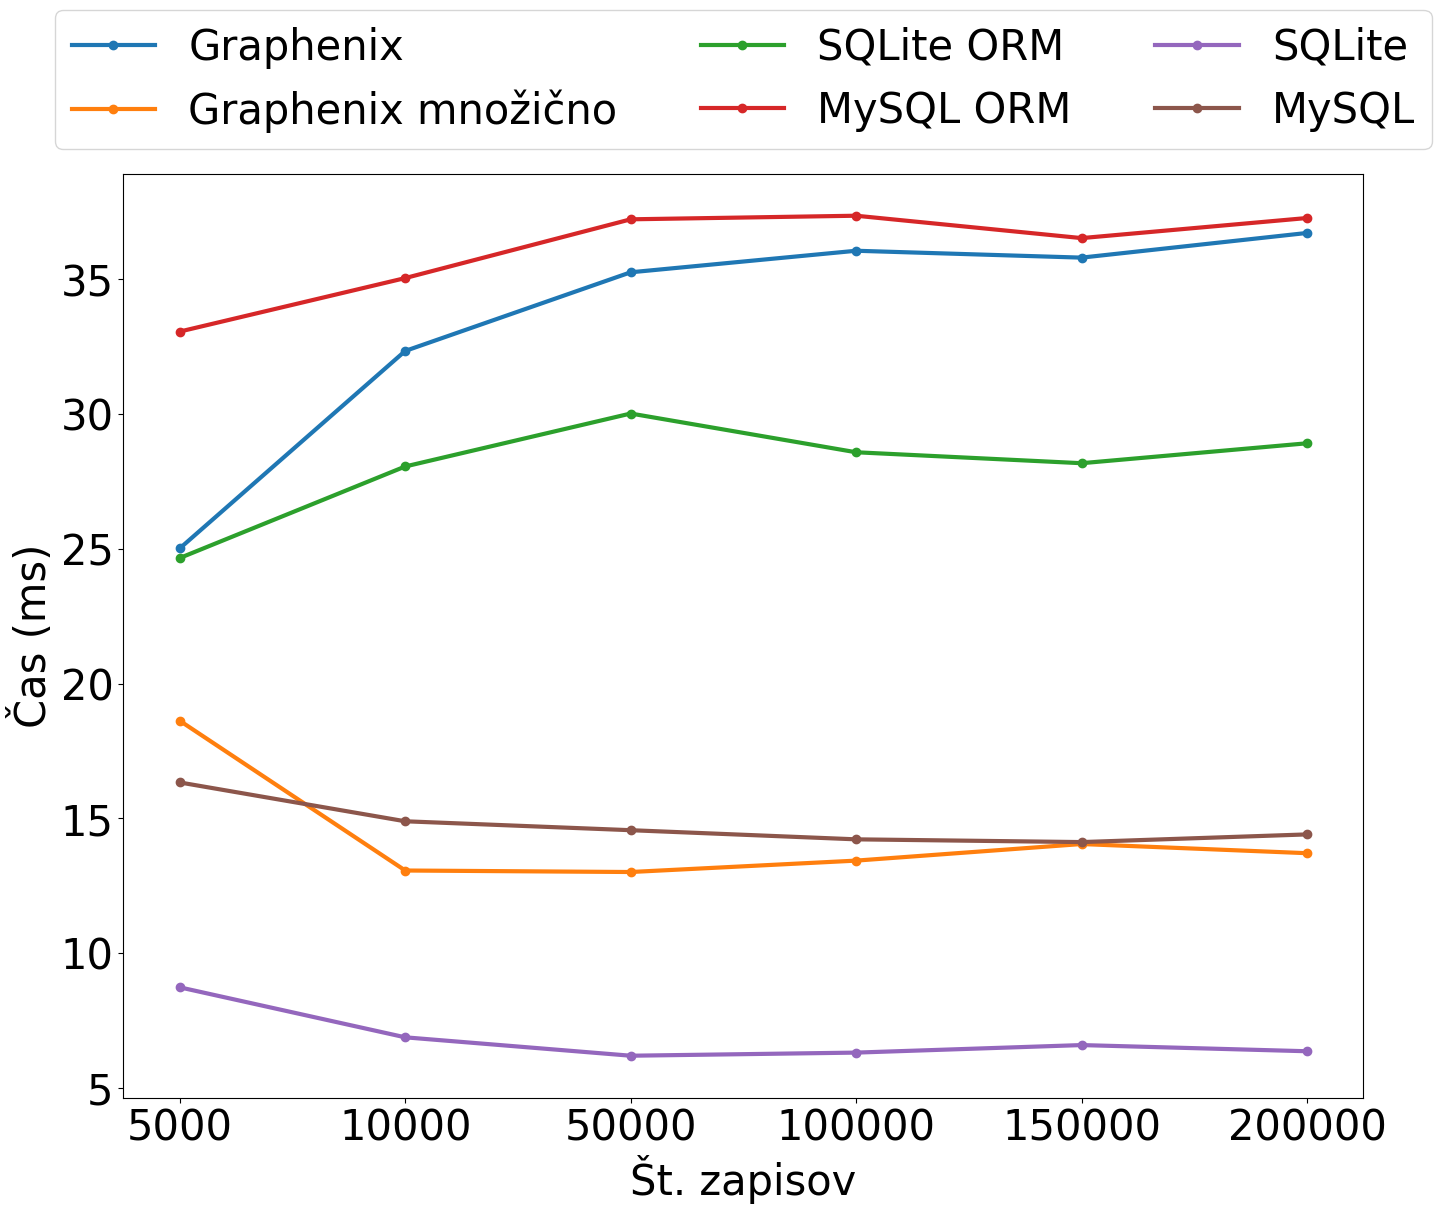
\includegraphics[width=0.77\textwidth, angle=0]{singleinsert.png}}
        \caption{Množično vstavljanje podatkov.}
        \label{vnos}
    \end{figure}

    \noindent
    Prva ugotovitev, ki jo lahko izpeljemo iz grafa~\ref{vnos} je, da je vstavljanje podatkov z uporabo ORM precej počasnejše v primerjavi z neposrednim vstavljanjem preko SQL ukazov. Uporaba ORM zahteva ustvarjanje instanc razredov, kar vodi v dodatne časovne zakasnitve.

    Na splošno lahko opazimo, da je SQLite prevladujoč pri hitrosti vstavljanja. Razlog, da MySQL ni tako hiter, je dokaj enostaven. MySQL teče na strežniku in vso komunikacijo opravlja preko vgrajenega protokola, kjer se podatki prenašajo z uporabo TCP/IP paketov, kar ni tako učinkovito, kot uporaba vhodno/izhodnih operaciji v SQLite.

    V primeru Graphenix, vstavljanje ni izvedeno v klasični množični obliki, saj je vstavljanje vsakega zapisa ločen dostop do datoteke. V analizi sta predstavljena dva pristopa vnašanja z uporabo Graphenix. V primeru množičnega vnašanja gre za direkten klic funkcije jedra za vnašanje podatkov in ne potrebujemo kreirati instanc razredov, kar je bilo tudi glavno ozko grlo pri vnašanju podatkov z uporabo ORM.

    Pomemben dejavnik pri vnašanju podatkov je tudi dodatna varnost, ki jo zagotavljata SQLite in zlasti MySQL. Oba sistema imata dnevnike za povrnitev (angl. \textit{rollback journal}), ki v primeru napake omogočata povrnitev celotne baze podatkov v stanje pred vnašanjem. Posledično v primeru napake ali prekinitve v Graphenix tvegamo imeti neveljavne zapise v bazi podatkov.

    \subsection{Vstavljanje z dodatnim indeksiranim poljem}

    V drugem scenariju gre za enakovredno vstavljanje prvemu, vendar z dodatkom uporabe indeksa na atributu tabele (indeks je definiran na celoštevilskem polju, kjer je vsaka vrednost unikatna).
    
    \begin{figure}[H]
        \centerline{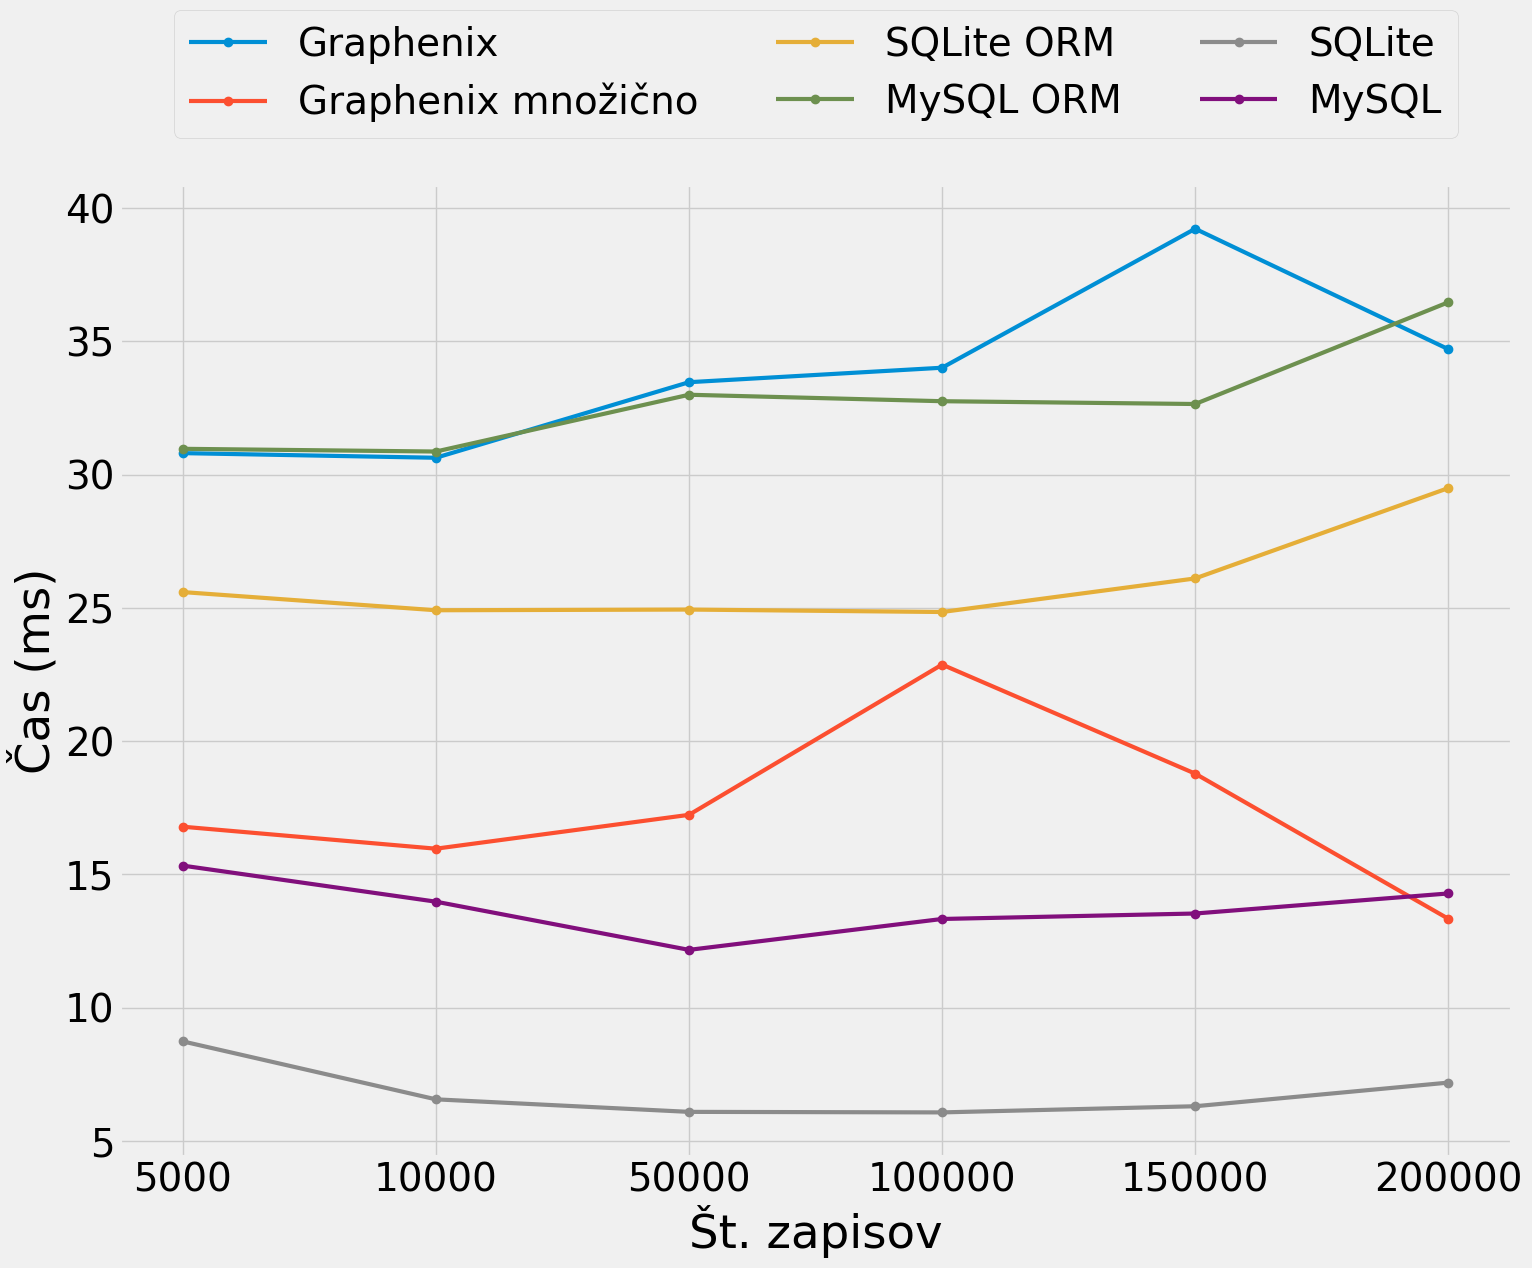
\includegraphics[width=0.77\textwidth, angle=0]{indexinsert.png}}
        \caption{Množično vstavljanje z dodatnim indeksiranim atributom.}
        \label{index_vnos}
    \end{figure}

    \noindent
    Iz grafa~\ref{index_vnos} lahko razberemo, da z vidika hitrosti vstavljanja še vedno prevladuje SQLite. Za razliko od predhodnega scenarija \ref{vnos}, pa je tokrat MySQL v večini primerov postal bolj učinkovit kot Graphenix.

    V vseh treh SUPB je indeksiranje realizirano z uporabo B drevesa. Kljub temu pa je razlika v načinu vstavljanja podatkov, saj naša implementacija B drevesa ne izkorišča algoritma za množično vstavljanje v drevo. MySQL in SQLite za vstavljanje uporabljata algoritem množičnega vstavljanja in posledično čas vstavljanja v drevo nima bistvenega vpliva na celoten čas vstavljanja.
 
    \section{Velikosti podatkovnih baz na disku}
    \label{size_analysis}

    Glede na prva dva scenarija smo pripravili tudi stolpčni grafikon \ref{velikosti}, kjer primerjamo porabo prostora na disku posameznega SUPB (gre za baze podatkov z $1 \times 10^6$ zapisi). 
    
    \begin{figure}[H]
        \centerline{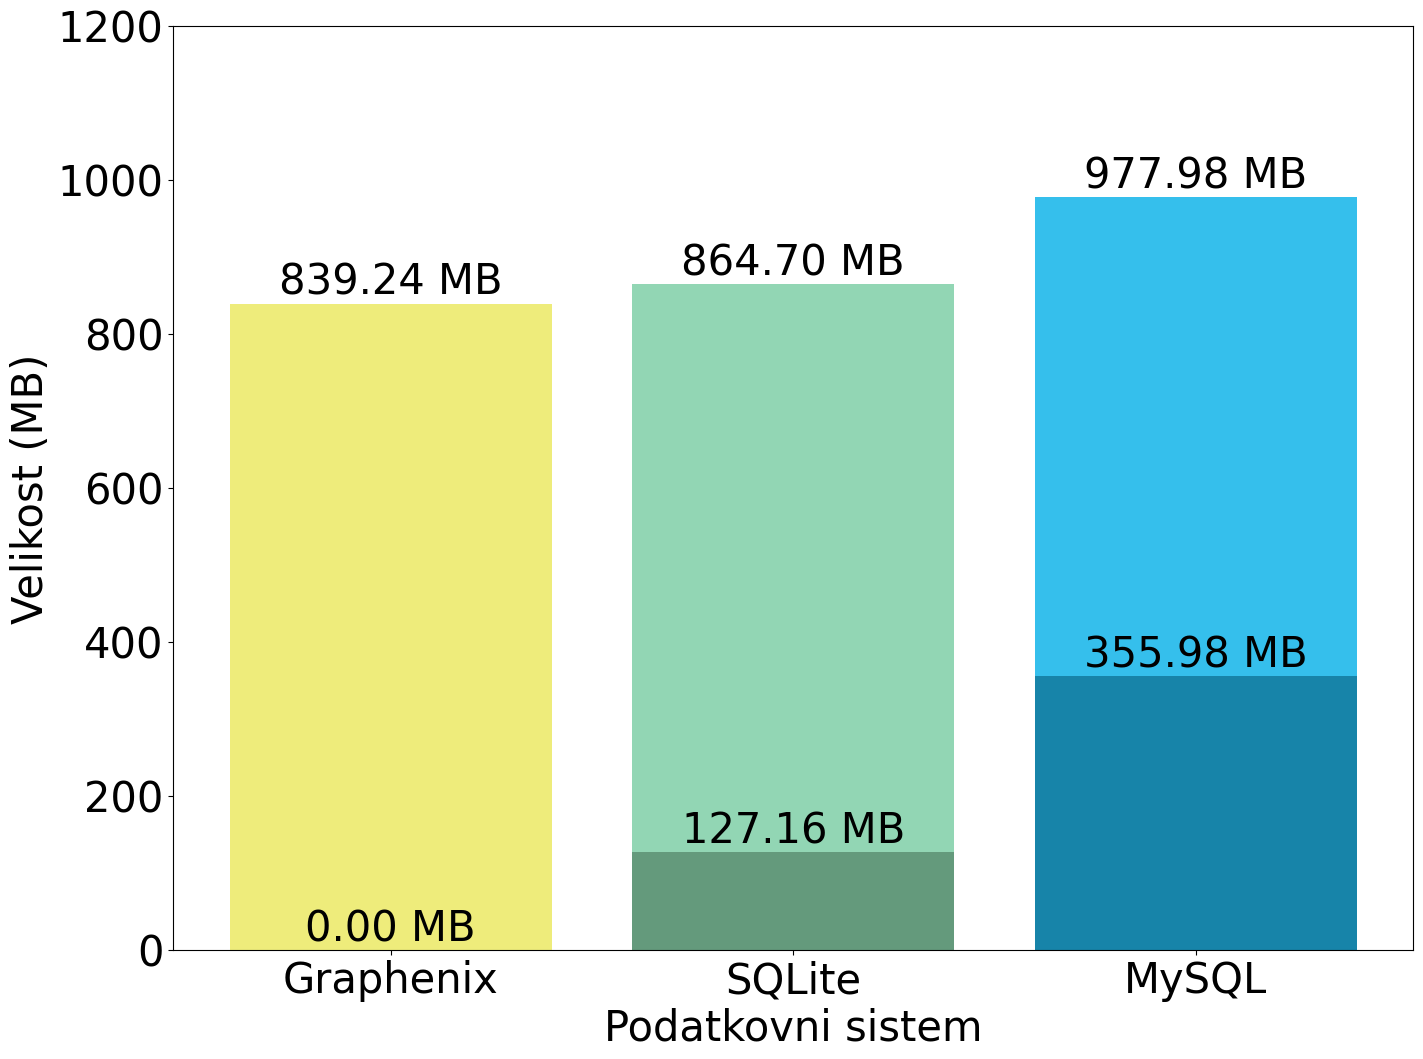
\includegraphics[width=0.7\textwidth, angle=0]{sizes.png}}
        \caption{Prostorska poraba na nivoju diska posameznega SUPB.}
        \label{velikosti}
    \end{figure}

    \noindent
    Iz grafa~\ref{velikosti} razberemo, da je Graphenix najbolj potraten z vidika porabe prostora. Razlog se skriva v načinu shranjevanja tekstovnih vrednosti. SQLite in MySQL uporabljata podatkovne strukture, ki ob shranjevanju prinesejo dodatno optimizacijo porabe prostora, saj uporabita le toliko prostora kot je potrebno. V primeru Graphenix, pa je dolžina tekstovnih polj točno določena, in v primeru, da polje definiramo kot {\tt String(size=50)}, vsak zapis ne glede na dolžino zavzame 50 bajtov.

    V temnem delu stolpca je prikazana razlika velikosti z in brez uporabe indeksne strukture. SUPB z najnižjo porabo prostora z vidika velikosti indeksne strukture je SQLite. Razlog za nižjo porabo se nahaja v velikosti posameznega vozlišča in algoritmu vstavljanja v drevo, ki vpliva tudi na delitev vozlišč tekom vstavljanja.

    \section{Primerjava poizvedb na eni tabeli}

    Za tretji scenarij je pripravljena analiza, kjer izmerimo čas izvajanja na preprosti poizvedbi branja brez kakršnihkoli omejitev.
    
\begin{minted}[breaklines]{SQL}
SELECT * FROM users
\end{minted}
    

    \begin{figure}[H]
        \centerline{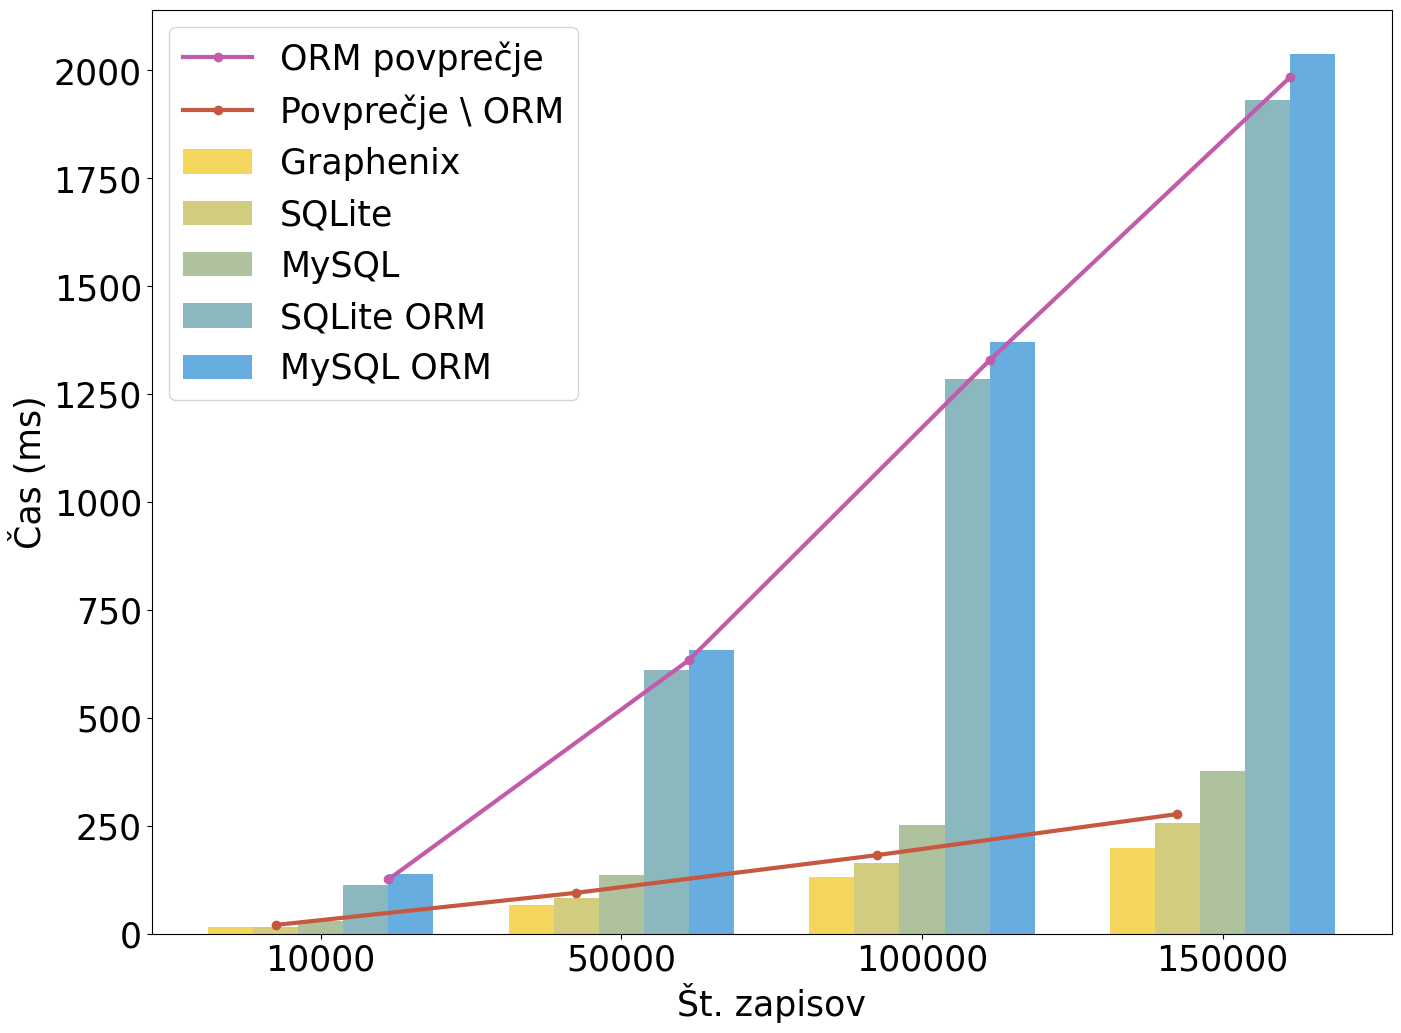
\includegraphics[width=0.75\textwidth, angle=0]{singleread.png}}
        \caption{Branje brez dodatnih parametrov znotraj poizvedbe.}
        \label{branje}
    \end{figure}

    \noindent
    Iz grafa~\ref{branje} je jasno razvidno, da uporaba ORM ni dobro pripravljena za masovno nalaganje podatkov, saj se ponovno kreirajo instance kar predstavlja več kot 70 \% delež celotnega branja. V primeru MySQL se ponovno pojavi tudi nekaj dodatne zakasnitve zaradi načina prenosa podatkov s TCP/IP protokolom.

    \subsection{Branje s filtriranjem, urejanjem in omejevanjem podatkov}

    V drugem scenariju branja podatkov iz ene tabele dodamo še omejitev na tip uporabnikov (želimo le administratorje). Poleg tega pa je dodano tudi urejanje podatkov in omejitev števila zapisov (želimo prvih 500 zapisov urejenih po točkah uporabnika).

\begin{minted}[breaklines]{SQL}
SELECT * FROM users WHERE is_admin = 1
ORDER BY points, id LIMIT 500
\end{minted}
    
    \begin{figure}[H]
        \centerline{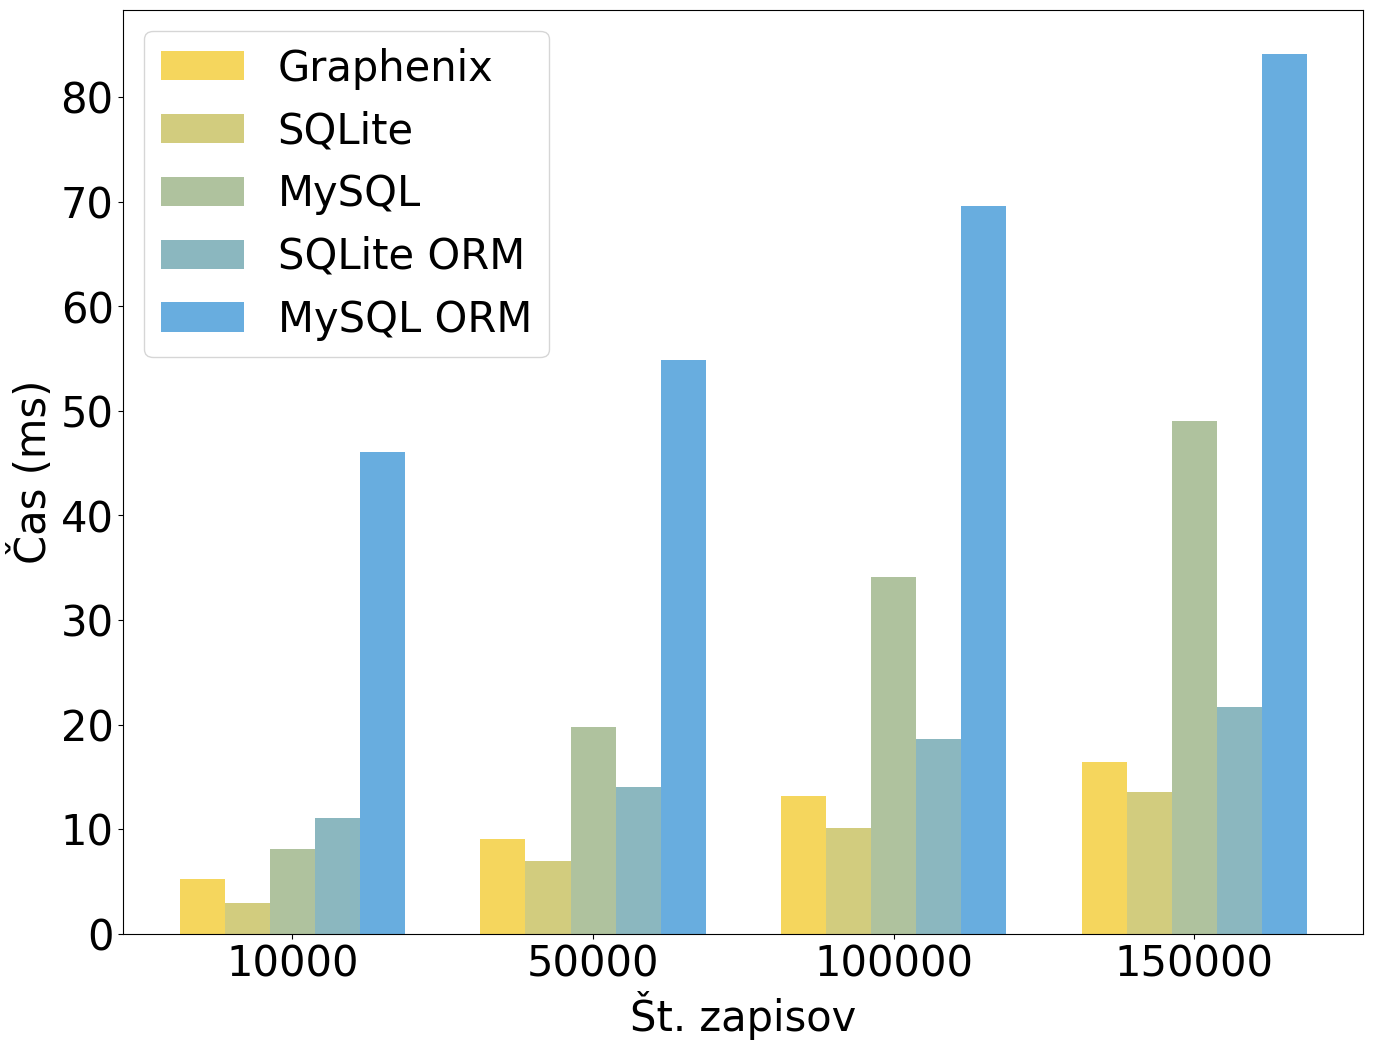
\includegraphics[width=0.72\textwidth, angle=0]{queryread.png}}
        \caption{Branje z dodanim filtriranjem in urejanjem zapisov.}
        \label{queryread}
    \end{figure}

    \noindent
    Čas izvajanja posameznega branja je relativno nizek, v vseh primerih je bilo branje izvedeno v manj kot 100 ms. Opazimo, da zakasnitve kreiranja instanc pri ORM tukaj ne pridejo do izraza, saj je potrebno kreirati le 500 instanc. Do večjega izraza pridejo zakasnitve, ki jih za prenos podatkov prinaša TCP/IP protokol, kar je na grafu~\ref{queryread} videno v primerih uporabe MySQL.

    \section{Primerjava poizvedb z uporabo relaciji}
    \label{join_lbl}

    V scenariju definiramo poizvedbo, kjer izvedemo nabor podatkov iz dveh tabel. Število zapisov je določeno s številom uporabnikov. Za vsakega uporabnika pa je bilo vnesenih še 10 nalog, ki so vezane preko tujega ključa {\tt user\_id} v tabeli nalog ({\tt Task}).
    
\begin{minted}[breaklines]{SQL}
SELECT * FROM users 
INNER JOIN tasks ON tasks.user_id = users.id
\end{minted}

    \begin{figure}[H]
        \centerline{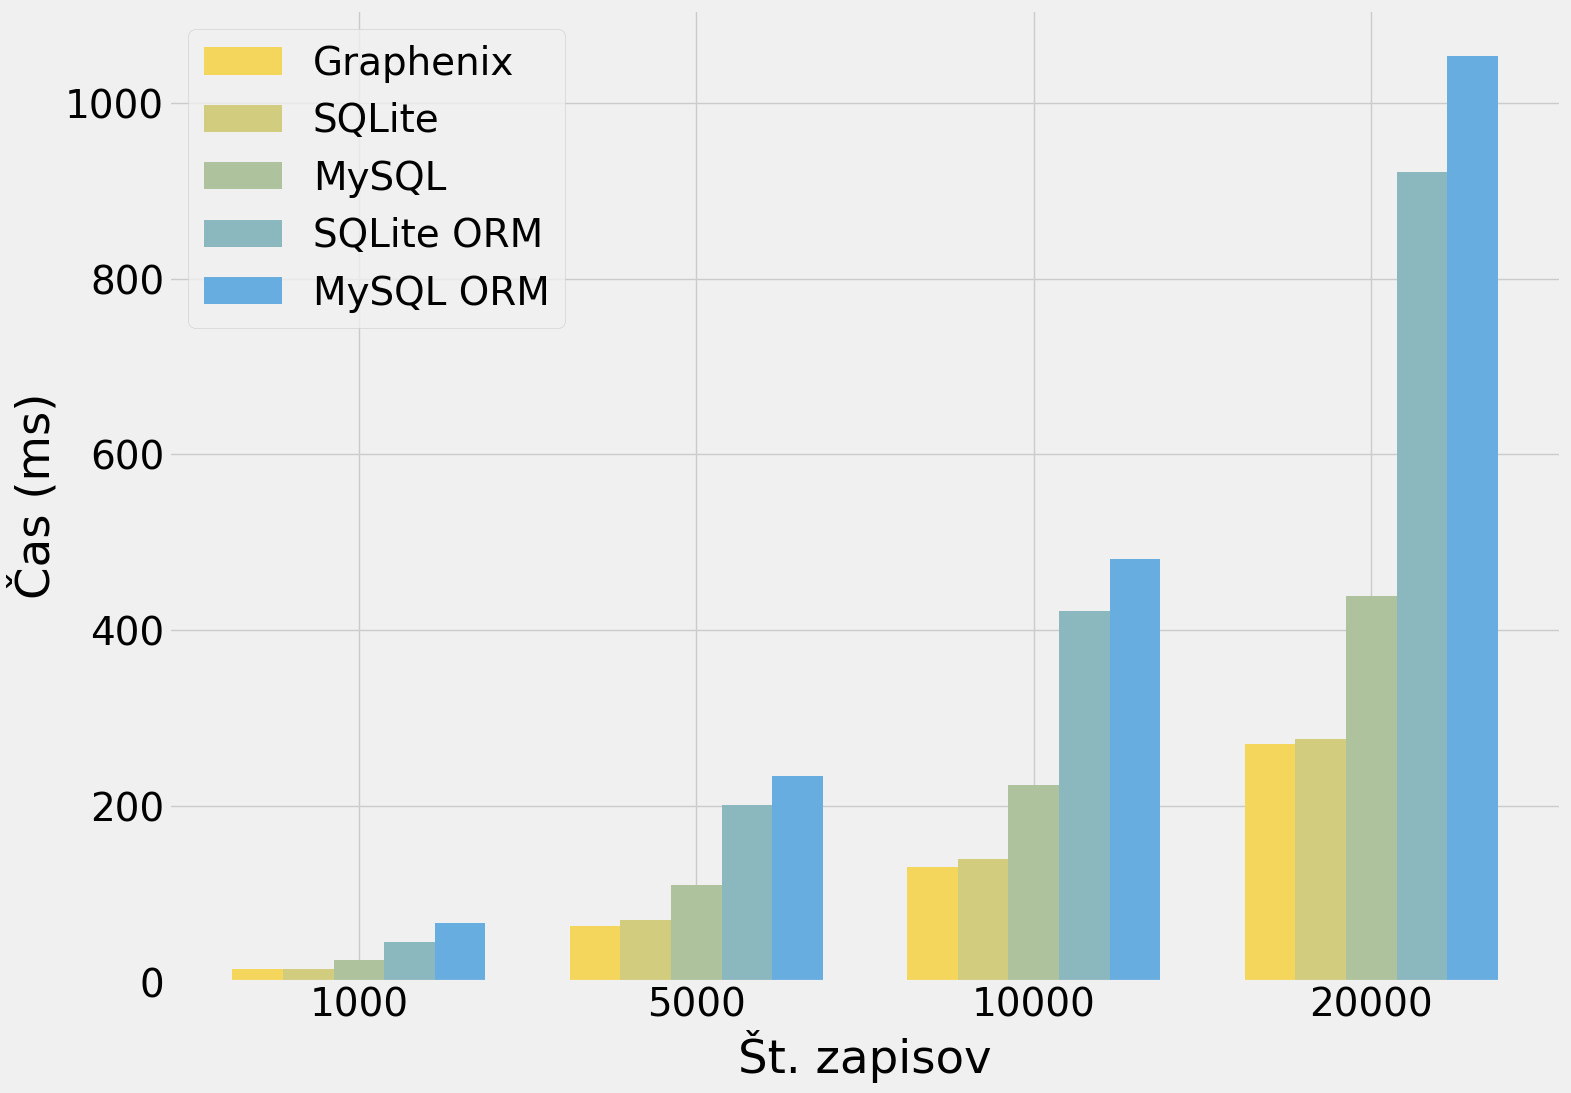
\includegraphics[width=0.72\textwidth, angle=0]{join.png}}
        \caption{Poizvedovanje podatkov iz dveh tabel hkrati – uporabniki in njihove naloge.}
        \label{join}
    \end{figure}

    \noindent
    Ponovno se izkaže, da ORM s seboj prinese dodatne zakasnitve zaradi kreiranja instanc. Za razliko od prejšnjih scenarijev pride tukaj do razlike v sami strukturi rezultata.
    
    \begin{itemize}
        \item ORM – podatki so v gnezdeni obliki, kjer imamo za vsakega izmed uporabnikov seznam njegovih nalog.
        \item Brez – podatki so predstavljeni v obliki matrike, kjer imamo za vsakega uporabnika toliko zapisov, kot ima uporabnik sporočil.
    \end{itemize}

    \noindent
    Graphenix deluje po principu ORM in imamo gnezdeno strukturo podatkov. Kljub temu pa zaradi združevanja na nivoju programskega jezika C++ poizvedba steče v primerljivem času s poizvedbami, ki ne uporabljajo ORM.
    
    \section{Izvedba agregacijske poizvedbe}

    V scenariju izvedbe agregacije uporabljamo strukturo, ki smo jo pripravili v prejšnjem scenariju \ref{join_lbl}.

    V poizvedbi naloge združujemo po uporabnikih in za vsakega uporabnika pridobimo število nalog, ki mora biti v vseh primerih 10. Poleg tega pa glede na atribut {\tt created\_at} pridobimo tudi datum zadnje naloge uporabnika.
    
\begin{minted}[breaklines]{SQL}
SELECT user_id, COUNT(*) AS 'count', 
       MAX(created_at) AS 'latest' 
FROM tasks GROUP BY user_id
\end{minted}

    \begin{figure}[H]
        \centerline{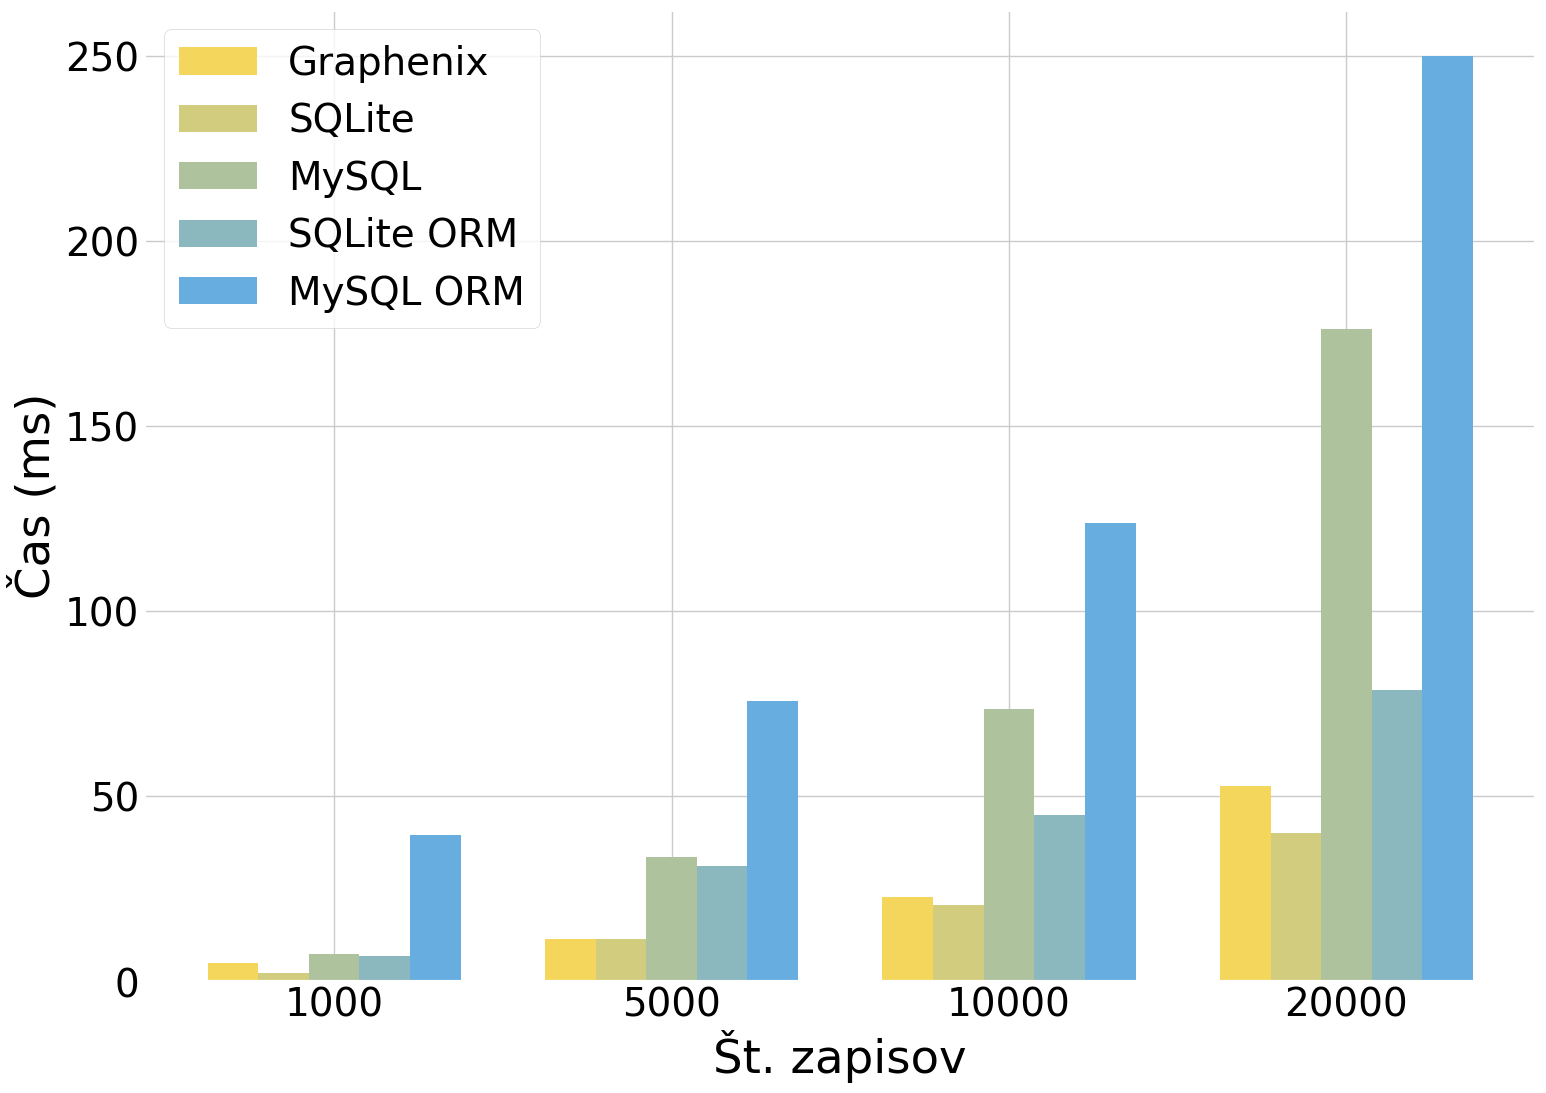
\includegraphics[width=0.75\textwidth, angle=0]{agg.png}}
        \caption{Uporaba agregacijskih metod.}
        \label{agg}
    \end{figure}

    \noindent
    V tem scenariju rezultat poizvedbe ni predstavljen kot instance razredov, saj vedno kreiramo prilagojen tip rezultata, ki vsebuje identifikator uporabnika, število nalog in zadnji datum naloge za vezanega uporabnika.

    Rezultati sicer dobro sledijo trendom iz predhodnih scenarijev – MySQL zaradi načina prenosa podatkov potrebuje nekoliko več časa, poleg tega pa se ponovno pozna razlika uporabe ORM in uporaba poizvedb SQL. Graphenix pa je ponovno primerljiv uporabi SQLite brez ORM.

    \section{Pohitritve s pomočjo indeksiranja}

    Kot zadnji scenarij je predstavljen eden izmed najbolj kritičnih segmentov SUPB – pohitritev iskanja s pomočjo indeksiranja podatkov. V scenariju primerjamo pristop brez in z uporabo indeksiranja.
    
\begin{minted}[breaklines]{SQL}
SELECT * FROM users
WHERE points = 5432
\end{minted}

    \noindent
    Na grafu \ref{old_speedup} je prikazano iskanje zapisa v tabeli z $ 1 \times 10^5$ zapisi.

    \begin{figure}[H]
        \centerline{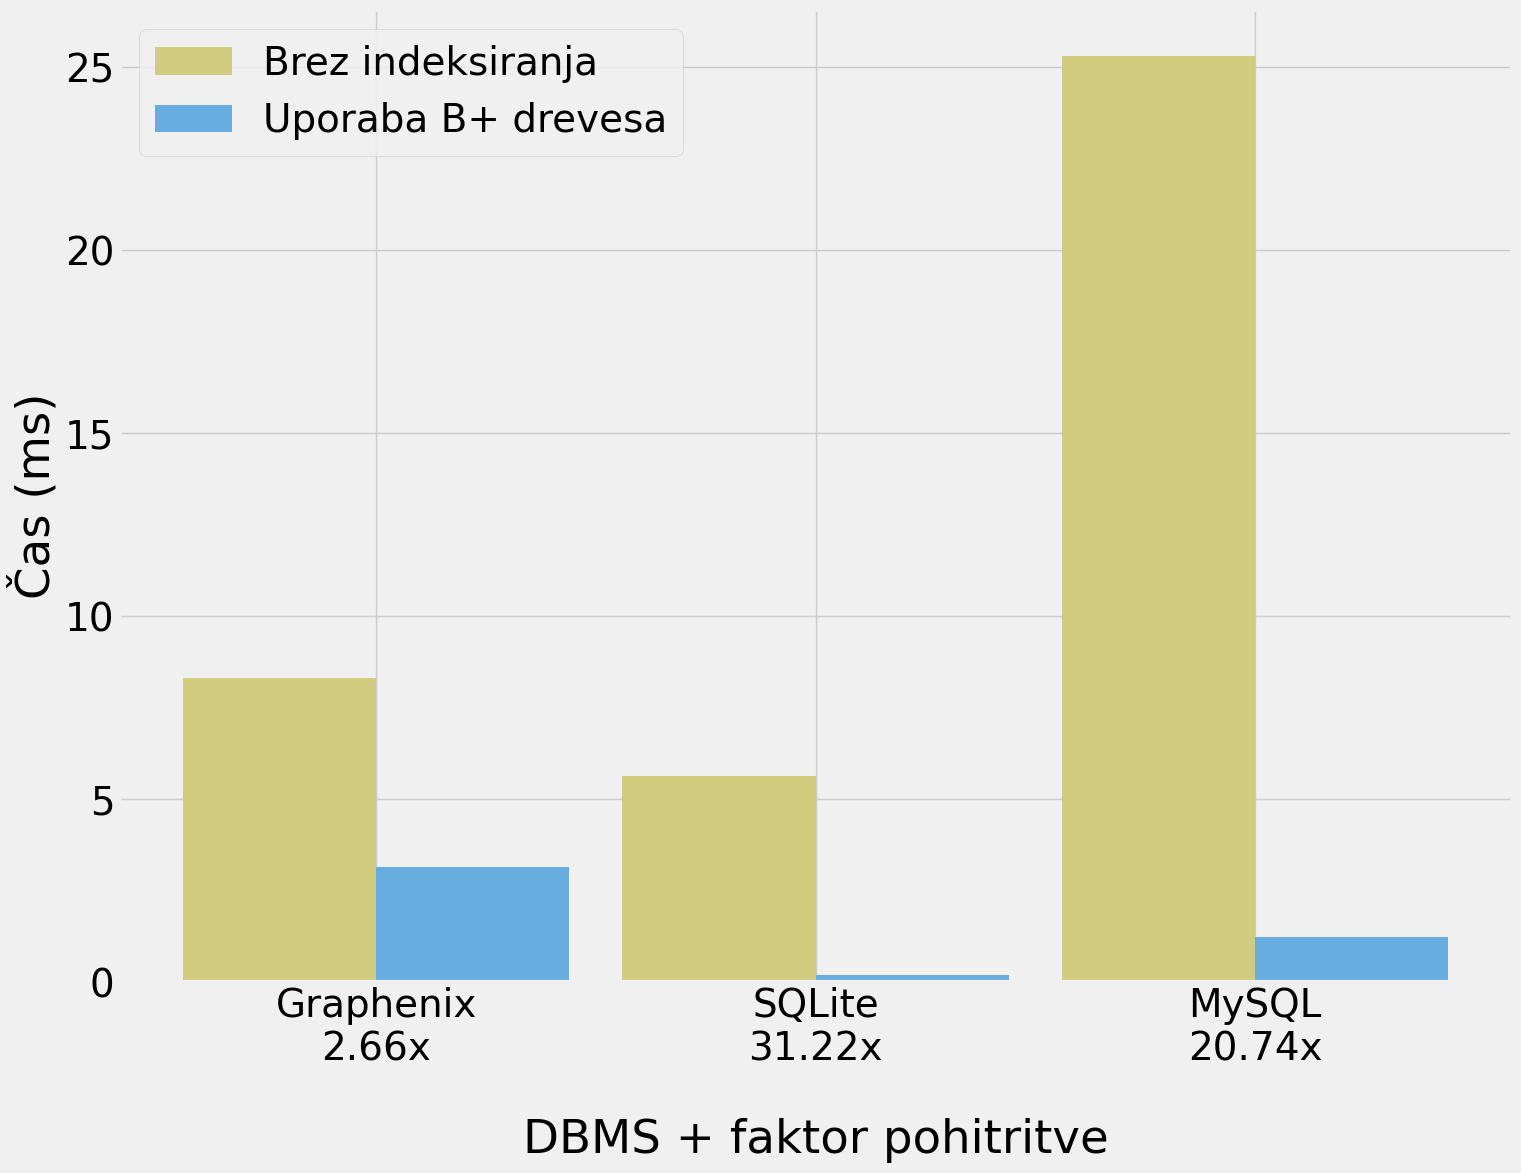
\includegraphics[width=0.8\textwidth, angle=0]{indexing_speedup_100000.png}}
        \caption{Iskanje specifičnega zapisa ($N = 1 \times 10^5$).}
        \label{old_speedup}
    \end{figure}

    \noindent
    Iz grafa~\ref{old_speedup} hitro razberemo, da je pohitritev v Graphenix SUPB drastično manjša, kot je to v primeru SQLite in MySQL.

    \subsection{Optimizacija v metodi filtriranja zapisov}

    Zaradi bistveno slabšega rezultata pri iskanju smo se lotili profiliranja posameznih segmentov programske kode za nabor podatkov.

    Kaj hitro smo prišli do ugotovitve, da težava ni bil proces iskanja v B drevesu, temveč je bila težava branje zaglavja tabele. Metoda za branje podatkov iz posamezne tabele je delovala tako, da je najprej prebrala celotno datoteko zaglavja tabele in za posamezen identifikator zapisa pridobila še odmik v matriki zapisov. Izkazalo se je, da je ta proces v scenariju predstavljal nekje $\approx 85$ \% izvajalnega časa.

    V namen hitrejšega izvajanja se branja celotnega zaglavja, v primeru, da imamo že vnaprej določene identifikatorje, ki jih iščemo in je teh manj kot {\tt IX\_THRESHOLD}, izognemo. Konstanta predstavlja mejo za branje celotnega zaglavja in je v trenutni implementaciji nastavljena na \num{100}.
    
    \begin{figure}[H]
        \centerline{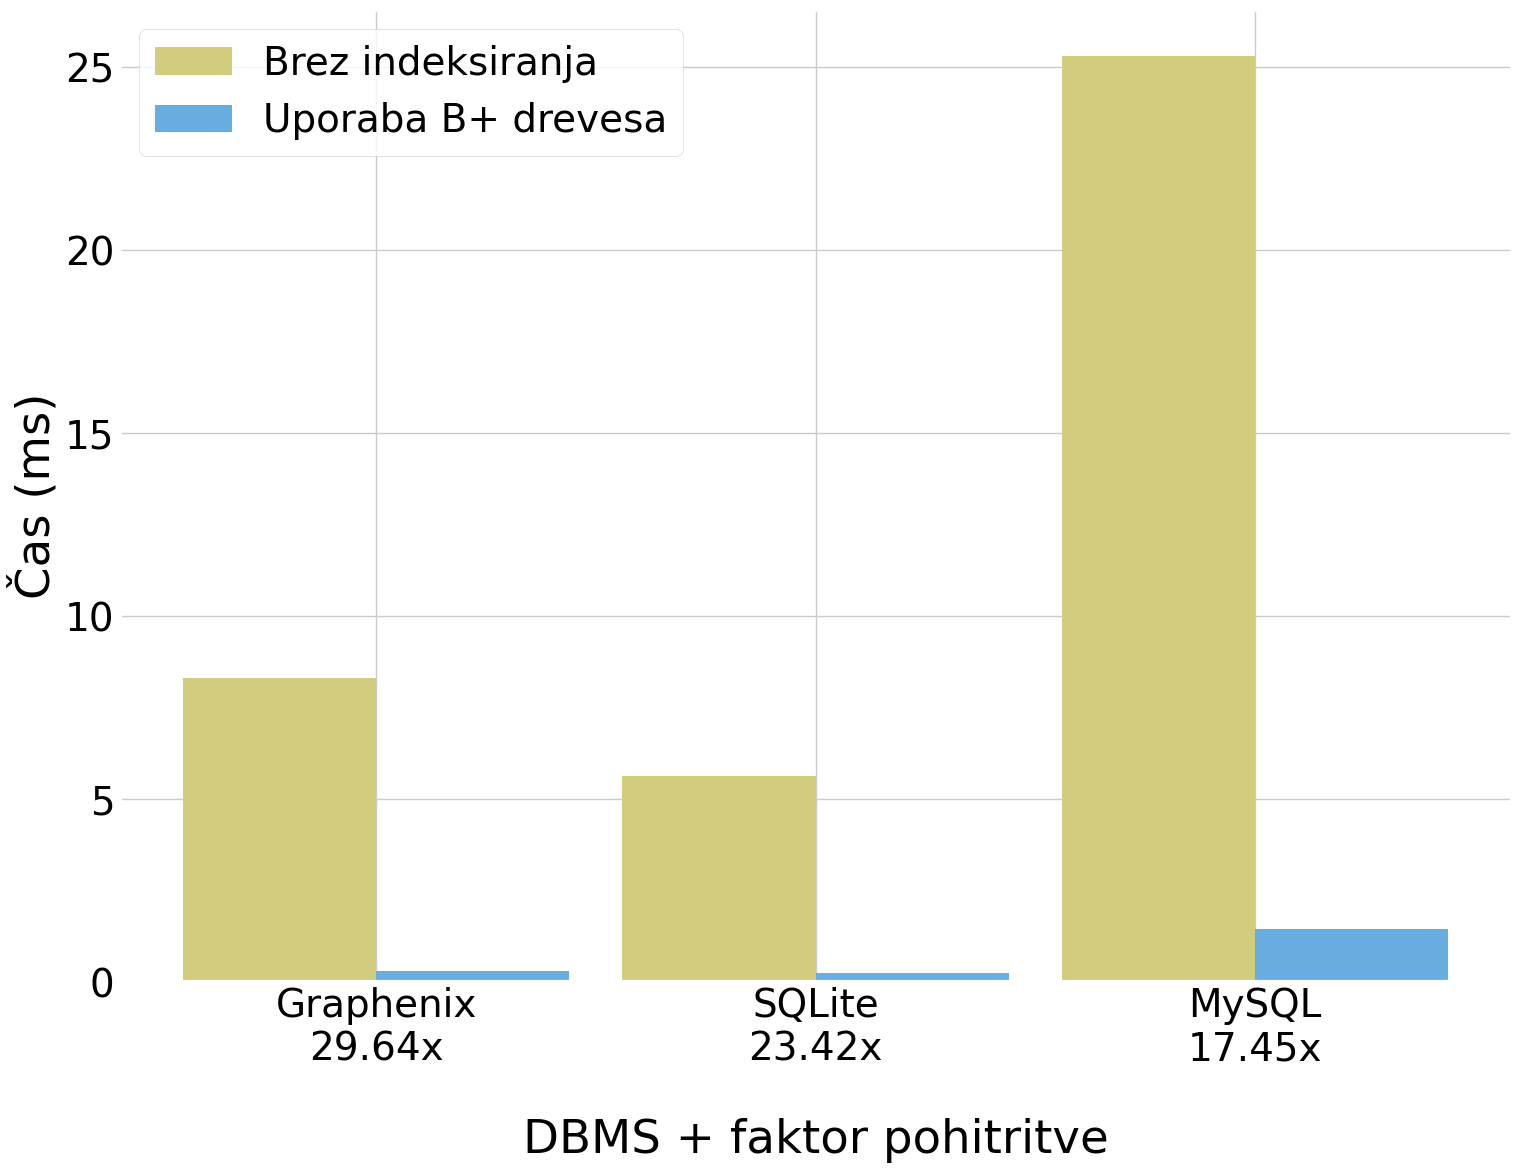
\includegraphics[width=0.8\textwidth, angle=0]{indexing_speedup_100000_v2.png}}
        \caption{Iskanje specifičnega zapisa ($N = 1 \times 10^5$) z optimizacijo.}
        \label{idx_speedup}
    \end{figure}

    \noindent
    Po implementirani optimizaciji opazimo bistveno izboljšavo časa iskanja. Sedaj se čas in faktor pohitritve lahko primerjata z MySQL in SQLite.

    \subsection{Analiza iskanja nad večjo bazo podatkov}

    Na grafu \ref{idx_speedup_2} je prikazana še pohitritev enake poizvedbe, kot v predhodnem scenariju. V tem primeru pa je število vseh uporabnikov $1 \times 10^6$.
    
    \begin{figure}[H]
        \centerline{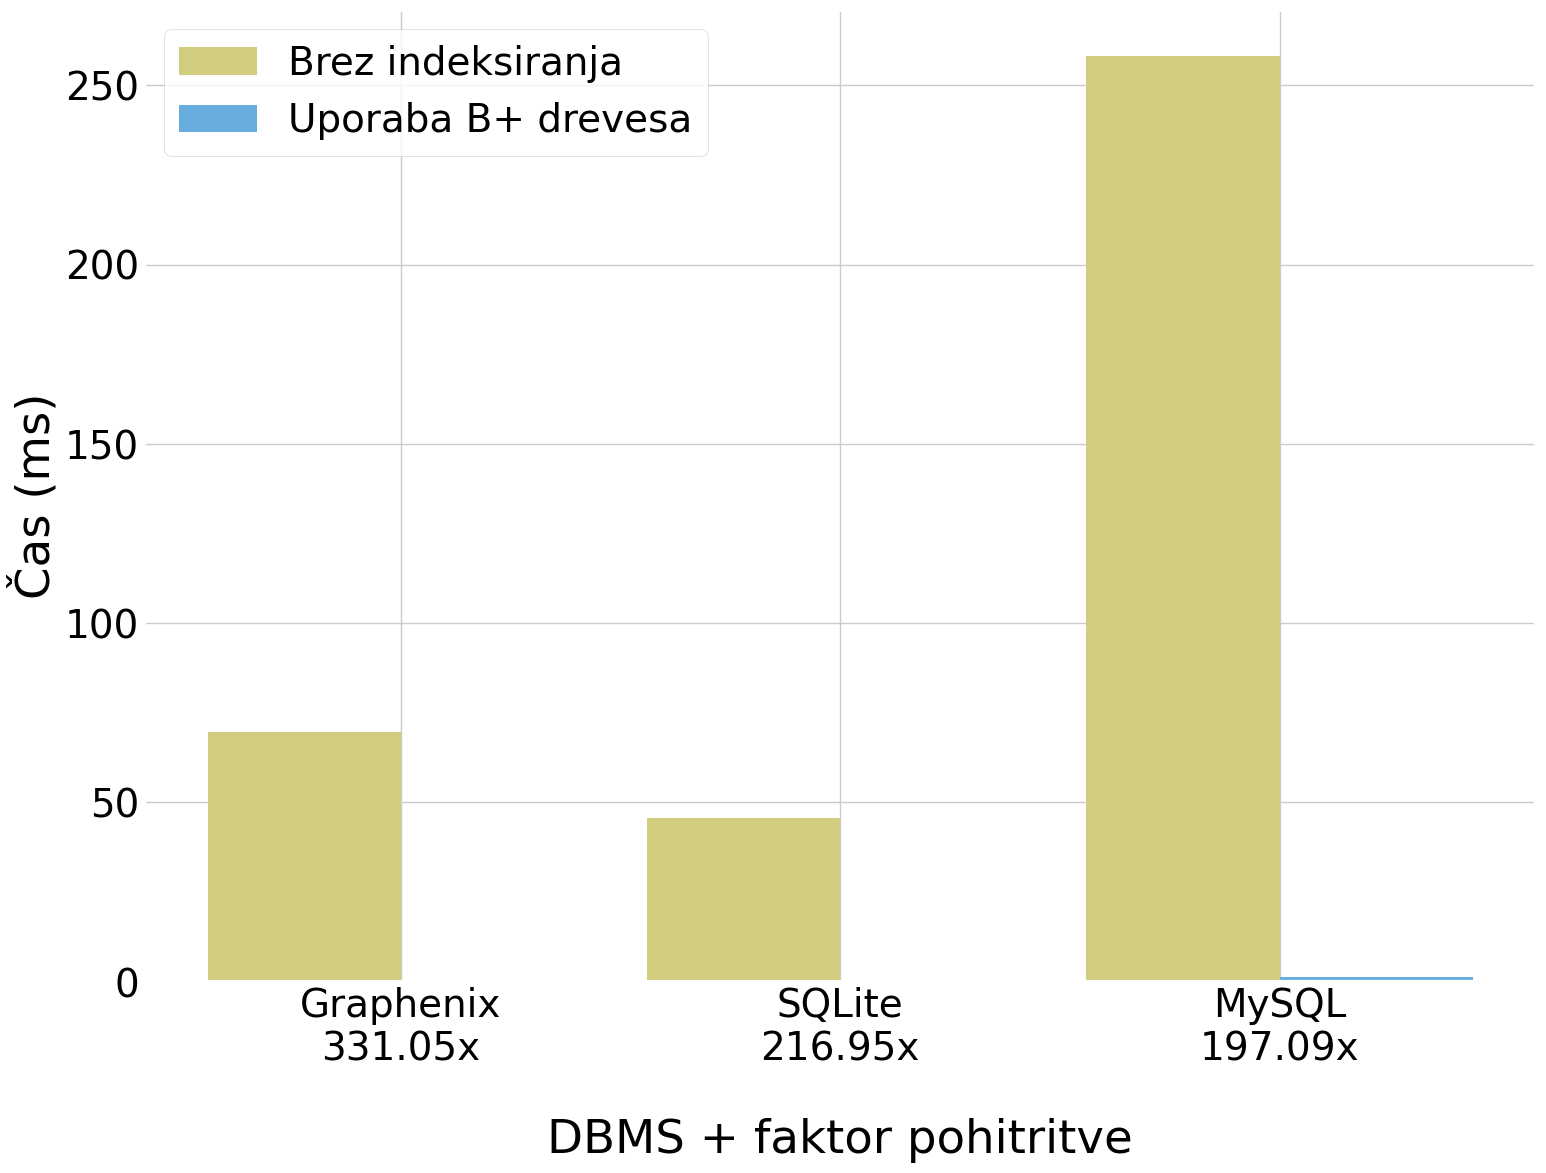
\includegraphics[width=0.8\textwidth, angle=0]{indexing_speedup_1000000_v2.png}}
        \caption{Iskanje specifičnega zapisa ($N = 1 \times 10^6$) z optimizacijo.}
        \label{idx_speedup_2}
    \end{figure}

    \noindent
    Iz grafa~\ref{idx_speedup_2} razberemo, da v vseh treh izvedbah zapis najdemo v manj kot 2 ms, kar tudi v vseh treh scenariji predstavlja več 100x pohitritev. Nekaj zakasnitve se sicer pojavi iz strani MySQL, kar je glede na predhodne scenarije pričakovano.

    \subsubsection{Idealni pogoji za indeksiranje}
    Omenimo, da je scenarij prilagojen uporabi indeksiranja, saj v scenariju iskanja, kjer vrednosti niso unikatne, učinkovitost indeksa zelo hitro pade. Poleg tega je bilo iskanje izvedeno kot iskanje specifične vrednosti v drevesu, medtem ko če bi iskali širši nabor vrednosti bi časovna zahtevnost $O(log_b(N))$ postala $O(K \cdot log_b(N))$, kjer je $K$ število vrednosti, ki se ujemajo z iskalnim kriterijem.

    Če potegnemo črto je jasno, da se pri odločanju o uporabi indeksov odpira zahtevno vprašanje, ki zahteva premišljeno obravnavo. Odgovornost za to odločitev se prepušča razvijalcem, pri čemer je ključnega pomena, da se kot razvijalci zavedamo optimizaciji in pasti, ki izvirajo iz uporabe B dreves za indeksiranje. Poleg tega je nujno, da poznamo naravo podatkov in zahtev aplikacije, saj je optimizacija z indeksiranjem smiselna le v določenih kontekstih.

\chapter{Scenariji oz. primeri uporabe}
\label{ch3}

    V tem poglavju sta predstavljena dva primera uporabe paketa Graphenix. V prvem primeru se paket uporablja kot dodatek strežniški aplikacij v namen beleženja podatkov (angl. \textit{logging}). V drugem scenariju pa je predstavljen razvoj preproste namizne aplikacije, kjer paket uporabljamo za trajno shranjevanje podatkov. Oba primera skušata na praktičen način predstaviti dobre strani uporabe rešitve Graphenix.

    \section{Strežniško beleženje podatkov}

    Pogosta uporaba programskega jezika Python je na strani strežniških aplikacij. Na tem področju je beleženje sprememb in zahtev kritično. Z uporabo pripravljene rešitve je prilagojeno beleženje podatkov lahko zelo preprosto.

    \subsection{Aplikacija, ki služi kot osnova za modul beleženja}

    V prvi fazi smo si za primer pripravili preprosto strežniško aplikacijo, ki uporablja Flask \cite{FLASK_GITHUB} ogrodje. Znotraj aplikacije smo definirali eno vhodno točko, in sicer {\tt get-range}, ki je predstavljena v programski kodi \ref{simple_flask_app}, kjer lahko poljubno nastavljamo tri HTTP {\tt GET} parametre, to so {\tt start}, {\tt end} in {\tt step}, kjer ima vsak od teh parametrov tudi privzete vrednosti.

\begin{code}
\begin{minted}{python}
app = Flask(__name__)
@app.route('/get-range')
def get_range(request):
    start = int(request.args.get('start', 0))
    end = int(request.args.get('end', 10))
    step = int(request.args.get('step', 1))
    return jsonify({'Range': list(range(start, end, step))})
app.run()
\end{minted}
\caption{Vhodna metoda za strežniško aplikacijo.}
\label{simple_flask_app}
\end{code}

    \subsection{Kreiranje sheme za beleženje podatkov}

    V namen beleženja podatkov smo si najprej pripravili tabelo in shemo za shranjevanje podatkov, kar je prikazano v programski kodi \ref{logging_schema}.

\begin{code}
\begin{minted}{python}
class ReqInfo(gx.Model):
    route = gx.Field.String(size=255)
    timestamp = gx.Field.DateTime().as_index()
    route_req = gx.Field.String(size=1024)
    route_res = gx.Field.String(size=1024)
    resp_code = gx.Field.Int()

logging = gx.Schema('logging', models=[ReqInfo])
if not logging.exists():
    logging.create()
\end{minted}
\caption{Shema za beleženje podatkov.}
\label{logging_schema}
\end{code}

    \noindent
    Tabela {\tt ReqInfo} skupaj z definiranimi atributi predstavlja strukturo podatkov, ki jih bomo tekom delovanja naše aplikacije beležili. V drugi fazi pa moramo kreirati še shemo, v kateri definiramo naziv in vse razrede oz. tabele, ki bodo del naše baze podatkov.

    \subsection{Dekorator za dinamično dodajanje beleženja}

    V namen beleženja znotraj vhodnih točk strežniške aplikacije smo uporabili pristop z uporabo dekoratorja.
    Dekorator je vzorec,  ki omogoča dinamično dodajanje funkcionalnost obstoječi funkciji, ne da bi spreminjali njeno strukturo. Med izvedbo notranje funkcije lahko argumente in različne segmente izvajanja prestrežemo in jih prilagodimo glede na naše zahteve \cite{mu2011design}.

\begin{code}
\begin{minted}[breaklines]{python}
def route_with_log(route):
    def decorator(f):
        @wraps(f)
        def wrapper(*args, **kwargs):
            try:
                response = f(request, *args, **kwargs)
            except Exception as err:
                response = None
            ReqInfo(
                route=route,
                timestamp=datetime.now(),
                route_req=json.dumps(dict(request.args)),
                route_res=response.get_data(as_text=True) if response else '',
                resp_code=response.status_code if response else 500
            ).make()
            return response
        app.add_url_rule(route, view_func=wrapper)
        return wrapper
    return decorator
\end{minted}
\caption{Dekotrator za implementacijo avtomatskega beleženja.}
\label{log_decorator}
\end{code}

    \noindent
    V primeru našega dekoratorja {\tt @route\_with\_log} vhodni točki dodamo še funkcionalnost beleženja podatkov.

    \subsection{Branje zapisanih podatkov}

    V končni fazi je glavna prednost uporabe pripravljene rešitve dobra struktura shranjenih podatkov, ki omogoča preprosto obdelavo in manipulacijo. Posledično nam je omogočeno tudi bistveno več načinov pridobivanja statističnih podatkov, saj lahko le-te poljubno filtriramo, grupiramo, združujemo in razvrščamo. Na nivoju administratorske aplikacije lahko nato prožimo različne poizvedbe nad našo bazo podatkov.

    \subsubsection{Izpis zadnjih treh zahtevkov}

\begin{minted}{python}
_, reqs = ReqInfo.order(ReqInfo.timestamp.desc()).limit(3).all()
... 
# izpis zahtevkov
ReqInfo(id=3, route=/get-range, timestamp=2023-07-16 03:02:15, 
    route_req={}, route_res={"Range":[0,1,2,3,4,5,6,7,8,9]},
    resp_code=200)
    
ReqInfo(id=2, route=/get-range, timestamp=2023-07-16 03:02:13, 
    route_req={"start": "3"}, route_res={"Range":[3,4,5,6,7,8,9]},
    resp_code=200)
    
ReqInfo(id=1, route=/get-range, timestamp=2023-07-16 03:02:05,
    route_req={"start": "15", "end": "10", "step": "-3"},
    route_res={"Range":[15,12]}, resp_code=200)
\end{minted}

    \newpage
    \subsubsection{Statističen pregled zahtevkov}

    Podatke lahko v pripravljenem SUPB tudi grupiramo, in sicer z uporabo {\tt .agg(...)} metode v poizvedbi. Znotraj metode definiramo polje po katerem grupiramo podatke, kot tudi agregacije, ki jih želimo izvesti.
    
\begin{minted}{python}
route_stats = ReqInfo\
    .agg(by=ReqInfo.route, count=gx.AGG.count())
\end{minted}

    \noindent
    S poizvedbo dobimo število zahtevkov grupiranih po vhodni točki aplikacije. 

    \subsubsection{Izpis napak v zadnjem dnevu}

    Za nabor napak v zadnjem dnevu, lahko preprosto izvedemo poizvedbo, kjer zahtevamo, da je status odgovora $>= 400$, kar pri zahtevkih, ki uporabljajo HTTP protokol, predstavlja razpon napak. Poleg tega pa dodamo še zahtevo, da mora biti datum napake večji, kot včerajšnji datum ob enaki uri. Na koncu zapise uredimo po datumu napake.

\begin{code}
\begin{minted}[breaklines]{python}
err_count, api_errors = ReqInfo\
    .filter(
        ReqInfo.resp_code.greater_or_equal(400),
        ReqInfo.timestamp.greater(
            datetime.now() - timedelta(days=1)
        )
    ).order(ReqInfo.timestamp.desc())\
    .all()
\end{minted}
\caption{Poizvedba za nabor napak v zadnjem dnevu.}
\label{api_errors_code}
\end{code}

    \subsubsection{Preslikava v podatkovne okvirje}

    Za namen podatkovne analitike v programskem jeziku Python najpogosteje uporabljamo rešitve, ki za svoje delovanje uporabljajo podatkovne okvirje. Ena taka rešitev je že omenjeni Pandas \cite{PANDAS_GITHUB}.
    
    Leta 2021 se je pojavil nov paket za podatkovno analitiko – Polars \cite{POLARS}. Za svoje delovanje uporablja prevedeni programski jezik, vendar v tem primeru ne gre za C/C++, temveč za programski jezik Rust \cite{RUST}.

    Prednost uporabe rešitve Graphenix za beleženje je v načinu branja podatkov, saj podatke zlahka filtriramo in urejamo že preden ustvarimo podatkovni okvir, kar klasične datoteke {\tt .csv}, ki pogosto predstavljajo format shranjenih podatkov, ne omogočajo.

\begin{code}
\begin{minted}{python}
import pandas as pd
import polars as pl

_, qview = ReqInfo.order(ReqInfo.timestamp)\
    .filter(ReqInfo.timestamp.greater_or_equal(
        datetime(2020, 1, 1)))\
    .limit(10000)\
    .all()

pandas_df : pd.DataFrame = qview.as_pandas_df()
polars_df : pl.DataFrame = qview.as_polars_df()
\end{minted}
\caption{Preslikava rezultata poizvedbe v podatkovna okvirja.}
\label{graphenix2pandas}
\end{code}

    \noindent
    V programski kodi \ref{graphenix2pandas} podatkovna okvirja napolnimo z zapisi, ki so bili ustvarjeni po začetku leta 2020 in od tega vzamemo prvih \num{10000} zapisov urejenih po datumu.

    Od te točke dalje pa lahko podatke v celoti obdelujemo s pomočjo paketov za podatkovno analitiko.

    \newpage
    \section{Namizna aplikacija za upravljanje stroškov}

    V tem razdelku je predstavljen razvoj namizne aplikacije za upravljanje stroškov. Aplikacija omogoča pregled stroškov, vstavljanje, urejanje, brisanje in statističen pregled, kjer so stroški grupirani glede na kategorije.

    \subsection{Zaslonski pregled aplikacije}
    Na sliki \ref{home_screen} je na levi prikazan začetni zaslon, kjer imamo v obliki seznama pregled vseh stroškov uporabnika in ob tem še zaslon za urejanje ali kreiranje novega stroška. 
    
    \begin{figure}[H]
        \centerline{\includegraphics[width=1\textwidth, angle=0]{app_psd.png}}
        \caption{Seznam stroškov z možnostjo vstavljanja in urejanja.}
        \label{home_screen}
    \end{figure}

    \noindent
    Za vsak posamezen strošek sta na skupnem prikazu definirani akciji za brisanje in urejanje. Poleg tega lahko stroške glede na naziv, ceno in kategorijo tudi uredimo. Omogočeno je tudi filtriranje po nazivu in prikazovanje po straneh.

    Na desnem zaslonu je prikazan obrazec, do katerega dostopamo preko akciji za urejanje in kreiranje novega stroška. Gre za preprost obrazec, kjer določimo naziv, ceno in kategorijo posameznega stroška.

    \subsubsection{Statističen pregled stroškov}
    Na sliki \ref{stats_screen} je prikazan statistični pregled stroškov, kjer so ti grupirani glede na kategorijo. Gre za tabelarni prikaz, kjer imamo za vsako kategorijo naziv, datum zadnjega stroška, število stroškov in vsoto cen vseh stroškov posamezne kategorije.

    \begin{figure}[H]
        \centerline{\includegraphics[width=1\textwidth, angle=0]{stats_psd.png}}
        \caption{Statističen pregled stroškov.}
        \label{stats_screen}
    \end{figure}

    \subsection{Aplikacija z vidika kode}

    Grahepnix je dobra izbira, saj gre za relativno nezahtevno aplikacijo, kjer ni potrebno skrbeti za več hkratnih dostopov do baze podatkov, poleg tega pa pripravljen ORM omogoča preprost pristop za manipulacijo podatkov.

    Za izris uporabniškega vmesnika aplikacija uporablja BeeWare \cite{BEE_WARE}, ki omogoča medplatformski (angl. \textit{Cross-platform}) razvoj programske opreme, kar pomeni, da lahko isto kodo uporabimo za več različnih operacijskih sistemov.

    \subsubsection{Struktura podatkovne baze}

    V namen beleženja stroškov je definiran razred {\tt Invoice}, kjer določimo naziv, ceno, datum in kategorijo posameznega stroška.
    Poleg tega pa imamo še tabelo, ki služi kot šifrant za kategorije stroškov. Podatki v kategorijah se napolnijo že ob kreiranju podatkovne baze z avtomatskim uvozom šifrantov.
    
\begin{code}
\begin{minted}{python}
class Invoice(gx.Model):
    title = gx.Field.String(size=20)
    amount = gx.Field.Int()
    day = gx.Field.DateTime()
    expense_type = gx.Field.Link()

class ExpenseType(gx.Model):
    name = gx.Field.String(size=30)
\end{minted}
\caption{Struktura za uporabo v namizni aplikaciji.}
\label{graphenix_schema_desktop}
\end{code}

    \subsubsection{Metoda za statistični nabor podatkov}

\begin{code}
\begin{minted}{python}
def refresh_stats(self):
    agg_data = Invoice.agg(by=Invoice.expense_type,
                           count=gx.AGG.count(), 
                           amount=gx.AGG.sum(Invoice.amount), 
                           latest=gx.AGG.max(Invoice.day))
    
    data = sorted(agg_data, key=lambda x: -x.amount)
    ...
\end{minted}
\caption{Metoda za osvežitev statističnega prikaza.}
\label{graphenix_refresh_desktop}
\end{code}

    \noindent
    V metodi \ref{graphenix_refresh_desktop} najprej izvedemo agregacijsko poizvedbo, kjer podatke grupiramo glede na kategorijo in pridobimo število zapisov, datum zadnjega stroška in vsoto cen pri posamezni kategoriji.

    Za zaključek podatke ločeno uredimo glede na skupno ceno, saj ta funkcionalnost za agregacijske metode v Graphenix SUPB ni podprta.

    \newpage
    \subsubsection{Nabor podatkov za glavni prikaz stroškov}

\begin{code}
\begin{minted}[breaklines]{python}
def display_expenses(self, search=None, order_by=None, page=0):
    query = Invoice.link(expense_type=ExpenseType).filter(
        Invoice.title.iregex(f'.*{search or ""}.*'))

    match order_by:
        case 'Title':
            query = query.order(Invoice.title)
        case 'Amount':
            query = query.order(Invoice.amount.desc())
        case _:
            query = query.order(Invoice.day.desc())
    
    _, invoices = query.offset(PAGE_SIZE * page)\
        .limit(PAGE_SIZE).all()
    
    for invoice in invoices:
        self.items_box.add(self.make_card(invoice))
\end{minted}
\caption{Metoda za nabor in prikaz stroškov.}
\label{graphenix_display_desktop}
\end{code}

    \noindent
    Za prikazovanje vseh stroškov uporabljamo metodo {\tt display\_expenses} \ref{graphenix_display_desktop}, ki prejme parameter za iskanje, urejanje in stran, ki jo mora prikazati. Prikazan je kodni vzorec grajenja (angl. \textit{builder pattern}), kjer postopoma dodajamo dodatne lastnosti na objekt poizvedbe. 
    \begin{enumerate}
        \item Na stroške povežemo kategorije in za iskanje uporabimo neobčutljiv {\tt regex} na male in velike črke, kjer pogoj zahteva, da naziv stroška vsebuje iskani niz {\tt search}.
        \item Parameter za urejanje preslikamo v določeno ureditev ali kot privzeto vrednost vzamemo padajoče urejanje po datumu.
        \item S pomočjo argumenta {\tt page} določimo stran, ki jo želimo prikazati. Nato v poizvedbi preskočimo {\tt PAGE\_SIZE} $\times$ {\tt page} stroškov, kjer je {\tt PAGE\_SIZE} konstanta, ki določa velikost strani. Hkrati pa dodamo še omejitev števila zapisov (vzamemo le prvih {\tt PAGE\_SIZE} zapisov).
    \end{enumerate}

    \noindent
    Za konec se le še sprehodimo skozi rezultat poizvedbe in za vsak strošek kreiramo element na uporabniškem vmesniku.
    

\chapter{Sklepne ugotovitve}
    
    V zaključenem poglavju so najprej na kratko predstavljene možnosti za izboljšavo paketa Graphenix, ki bi rešitev približale nivoju, ki je potreben za uporabo v produkcijskem okolju.

    V razdelku \ref{refleksija} pa je na kratko opisana celotna izkušnja razvoja programske rešitve.
    
    \section{Nadaljnji razvoj}

    Glede na širino področja upravljanja podatkovnih baz imamo na voljo obsežen spekter izboljšav. V okviru našega dela smo našli številne možnosti za nadgradnjo, ki bi lahko obogatile funkcionalnost in zmogljivosti celotne rešitve.
    
    \begin{enumerate}
        \item \textbf{Izboljšane indeksiranja}
        \newline
        \noindent
        Indeksiranje je v razviti programski opremi sicer implementirano in doseže primerljive rezultate z uveljavljenimi sistemi za upravljanje baz podatkov, ki smo jih vzeli za primerjavo.

        Kljub temu pa ostaja še ogromno scenarijev, ki jih z našo implementacijo nismo podprli. To je najbolj razvidno v množičnih akcijah, kot npr. iskanje več zapisov in množično vstavljanje v B+ drevo.

        \newpage
        \item \textbf{Prostorska optimizacija shranjevanja nizov}
        \newline
        \noindent
        Iz prostorske analize v razdelku \ref{size_analysis} je razvidno, da tako MySQL kot tudi SQLite ponujata prostorsko optimizacijo pri shranjevanju nizov.
        \begin{itemize}
            \item SQLite nize definira s podatkovnim tipom {\tt TEXT}, ki besedilo shranjuje v ločeni strukturi od zapisov in po potrebi zapise v tej ločeni strukturi premika.
            \item MySQL ima možnost uporabe podatkovnega tipa {\tt VARCHAR} \cite{MYSQL_VARCHAR}, kjer lahko definiramo maksimalno dolžino niza. Ta dolžina ne pomeni dejanske dolžine, ki jo niz porabi na disku, temveč MySQL SUPB izvaja dinamično alokacijo za nize. Uporabljen mehanizem s seboj poleg boljše izkoriščenega prostora na disku prinese tudi nekaj dodane zahtevnosti in dodatnih korakov za branje takih zapisov.
        \end{itemize}
    \end{enumerate}
    
    \section{Refleksija razvoja}
    \label{refleksija}

    Glavni cilj celotnega diplomskega dela je bila implementacija lastnega relacijskega sistema za upravljanje s podatkovno bazo, kjer bi na praktičen način spoznali ozadje delovanja relacijskih podatkovnih baz in obenem izdelali celovito rešitev za programski jezik Python.

    Razvoj dobrega SUPB ni lahka naloga, kar lahko razberemo iz količine programske kode in različnih konceptov, ki jih uporablja npr. odprtokodni MySQL \cite{MYSQL_GITHUB}.
    
    Spoznali smo, kako organizirati podatke za učinkovito izvedbo vseh operacij CRUD (ustvarjanje, branje, posodabljanje in brisanje). Za uspešno izvajanje je ključnega pomena tudi dobro poznavanje operacijskega sistema in načina, kako mehanizmu za shranjevanje omogočiti optimalno delo z datotekami.
    
     Poudarek je bil tudi na implementaciji indeksiranja z uporabo B+ drevesa. S tem smo uporabnikom paketa Graphenix omogočili možnost uporabe indeksov, ki ob določenih pogojih (v poizvedbi uporabljamo iskanje) bistveno pospešijo poizvedbe. Zagotovo gre za najbolj zapleten del celotnega sistema. Implementacija B+ drevesa je realizirana z rekurzivno strukturo in uporabo kazalcev, kjer smo implementirali tudi shranjevanje strukture v datoteko. Za naslednje različice pa smo identificirali možne izboljšave, ki bi pohitrile mehanizem indeksiranja.
    
    Poleg tega smo tekom razvoja dodali še lasten ORM, ki neposredno komunicira z operacijami SUPB, kar bistveno zmanjša zahtevnost, ki jo sicer prinese ORM, kjer moramo skrbeti še za dodatne preslikave med objekti in poizvedbami SQL. Pri združevanju zapisov iz različnih tabel smo se delno oddaljili od relacijskih podatkovnih baz in uporabili objektne pristope, ki jih uporabljajo nerelacijske podatkovne baze.
    
    Razvoj prototipa je bil uspešen. Z vključitvijo testnih primerov smo poskrbeli za hitrejše sprotno odkrivanje napak in višjo kakovost rešitve. Analiza uspešnosti je v nekaterih scenarijih pokazala celo primerljive rezultate z MySQL in SQLite, kar je bil tudi eden izmed glavnih ciljev pred začetkom razvoja.

%\cleardoublepage
% \addcontentsline{toc}{chapter}{Literatura}

% če imaš težave poravnati desni rob bibliografije, potem odkomentiraj spodnjo vrstico
\raggedright

% v zadnji verziji diplomskega dela običajno združiš vse tri vrste referenc v en sam seznam in
% izpustiš delne sezname
\printbibliography[heading=bibintoc,title={Literatura}]

\end{document}